%
% TU/e Style Master Thesis template for LaTeX
%
% Public version 1.0
% 2010 - 2013 Thijs Nugteren and Joos Buijs
%
% THIS IS THE MAIN FILE (i.e. compile this file, compiling the others directly won't work)
%
\documentclass[a4paper,10pt,twoside]{report}

%all the other includes etc. are done in the thesis.sty file.
\usepackage{thesis}

\newcommand{\abbr}[2]{\noindent{\bf #1} \enspace #2\\}
\newcommand{\X}{\text{\sffamily X}}

%
% These commands need to be defined in order to produce a correct and personalized document
%
\newcommand{\shortdoctitle}{Master's Thesis}
\newcommand{\doctitle}{SIMD Compiler Made Explicit in LLVM}
%\newcommand{\docsubtitle}{Master Thesis}
\newcommand{\docsubtitle}{Preparation Report}

\newcommand{\me}{Guus Hendrikus Peter Leijsten}
\newcommand{\keywords}{Compilers, SIMD, LLVM, Embedded Systems, Power Efficiency, Explicit Bypassing}
\newcommand{\version}{Draft version}
\newcommand{\monthYear}{March 2017}

%Be sure to use all the titles for your committee members!!! (their names show up on the very first page!)
\newcommand{\firstCommitteeMember}{Prof. dr. ir. Henk Corporaal}
\newcommand{\secondCommitteeMember}{Dr. ir. Roel Jordans}
\newcommand{\thirdCommitteeMember}{Ir. Luc Waeijen}
\newcommand{\fourthCommitteeMember}{Dr. ir. Lech Jozwiak}
%\newcommand{\fifthCommitteeMember}{Prof. dr. ir. Kees van Berkel}
\newcommand{\fifthCommitteeMember}{Dr. ir. Pieter Cuijpers}

\author{\me}

%
% PDF settings
%
\hypersetup
{
    pdfauthor={\me},
    pdftitle={\shortdoctitle},
    pdfsubject={\doctitle},
    pdfkeywords={\keywords}
}

\begin{document}

%use this include for PDF and distribution versions
\pagenumbering{roman}
\begin{titlepage}
\begin{center}

\includegraphics[height=2cm]{figures/tue-logo-high}\\
%\LARGE
%Eindhoven University of Technology \\
\large
Department of Electrical Engineering \\
Electronic Systems Group

\vspace*{10cm}

\setlength{\TPHorizModule}{1mm}
\setlength{\TPVertModule}{\TPHorizModule}
% Set the Paragraph Indent to zero, so the first line is not Indented
% Back-up the current value so it can be put back at the end of the title page
\newlength{\backupparindent}
\setlength{\backupparindent}{\parindent}
\setlength{\parindent}{0mm}			
% Begins a textbox at 72 mm from the left of the edge of the paper and 89 mm from the top
% The width of the textbox is 95 mm (167 - 72 mm)
% The height of the box cannot be defined, so it is your task to keep the text not too long
\begin{textblock}{95}(62,89)
    \vspace*{1mm}
    \huge
    \textbf{\doctitle \\}
    \Large
    \vspace*{5mm}
    \textit{\docsubtitle}\\
    \vspace*{10mm}
    \Large
    \me\\
\end{textblock}

\large
Committee:\\
\begin{tabular}{rl}
    \firstCommitteeMember\\
    \secondCommitteeMember\\
    \thirdCommitteeMember\\
    \fourthCommitteeMember\\
    \fifthCommitteeMember\\
\end{tabular}

\vfill
\version

\vfill
%\docdate \\
\large
Eindhoven, \monthYear\\

% Put the Paragraph Indent back to its original value
\setlength{\parindent}{\backupparindent}
\end{center}
\end{titlepage} 

\normalsize

\clearemptydoublepage

%Sometimes line numbers are nice, uncomment the next line to enable:
%\linenumbers

\chapter*{Abstract}\label{chapter:abstract}
%Old abstract
%In this report, we will research in ways to reduce energy consumption. We will achieve this by reducing the total amount of accesses to the register file by means of exploiting explicit datapaths. We describe six different approaches and evaluate which is most suitable based on tradeoffs, i.e. implementation complexity, compile time, quality of resulting code, etc. We have already implemented one approach. However, to improve it, and to handle vector instructions, we need to extend this work significantly. The real work begins only now. 

%New abstract

%TODO: extend abstract; its way too short
% abstract should not exceed 800 words.

This thesis describes the design of a code generator for a configurable programmable platform implementing an ultra-wide \emph{Single Instruction Multiple Data} (SIMD) architecture with explicit datapaths. The distinguishing characteristic of this architecture is a wide array of \emph{Processing Elements} (PEs) that exploit parallelism by processing many operations concurrently. Therefore, a high throughput can be achieved at a low clock frequency and thus low voltage, thereby with a high energy efficiency.

A LLVM-based compiler that targets this architecture exists, but lacks support for configurable explicit datapaths. This compiler is implemented completely within LLVM because it provides auto-vectorization that does support a configurable array size%LLVM is a collection of modular and reusable compiler and toolchain technologies that is popular amongst many companies for its multistage compilation strategy, outstanding extendability and maintainability. 
 
This work has a focus on extending the compiler with explicit bypassing capabilities. Explicit bypassing consists of two compiler optimizations, e.g. operand forwarding and dead result elimination. With operand forwarding, a value or result of an operation is forwarded from a pipeline stage to the \emph{Instruction Decode} stage, thereby, bypassing the \emph{Register File} (RF). When all consumers of a variable obtain it using forwarding, it is never read from the RF. Therefore, that variable does not need to be stored in a register file, since it is not read from it anyway. Dead result elimination (which is possible with explicit bypassing) consists of avoiding such redundant store accesses. With implicit bypassing the hardware performs bypasses automatically, while it is the compilers responsibility to find and allocate bypasses with explicit bypassing.

Compiling with explicit datapaths has been an active topic of research and several architectures face similar challenges. The \emph{Transport Triggered Architecture} (TTA) effectively faces the same challenge, except that compilation for TTAs is even more challenging because the datapaths is exposed in the instruction set. What TTAs have in common with code generation for SIMD with explicit datapaths is that explicit reads and writes are explicitly stated in the instruction set.

Several approaches to support explicit datapaths for the target SIMD architecture within LLVM have been ranked on implementation effort and expected results. Subsequently, one approach has been implemented and the efficiency of the generated code was accessed based on simulation results. 

With explicit bypassing, around 40\% of the accesses can be avoided. Since the RF consumers around 35\% of the total energy consumption and around 40\% of the communication with the RF can be avoided, an estimated improvement of around 15\% follows.

\vspace{10mm}
\noindent {\bf Keywords:} \keywords

%\clearemptydoublepage

%\chapter*{Preface}\label{chapter:preface}
%Before starting, I would like to take this opportunity to express my gratitude. I would like to thank all the people that are close to me for their continuous support and motivation to study electronic and computer systems. I want to thank my mom who is always there for me and my brother who always helps me in many ways. I would like to thank the ES-group for the project and for the many meetings that were hold over the duration of this project.

%Please write all your preface text here. If you do so, don't forget to thank your supervisor, other committee members, your family, colleagues etc.\ etc. 
Furthermore, I would also like to thank the leading expert on computer architectures at the TU/e, professor dr. Henk Corporaal for guidance and introducing me to the field. %introduced %intrigued TODO: Q: intrigued or introduced..? both are very ince 									 me to study computer architectures
Many thanks also go to my supervisor from Radbound university in Nijmegen, dr. ir. Roel Jordans for guidance and help on the compiler, and for introducing me to compilers.

Also, many thanks go to ir. Luc Waeijen who assisted me in many ways on technical aspects of this master project and to dr. ir. Lech Jozwiak, who always helps a lot by providing extremely useful feedback.

More thanks go to dr. ir. Pieter Cuijpers for joining my committee, and I would like to thank Liu Zhenyuan for his initial implementation of the compiler and Boyan Liang for his view on the hardware side of this project.

Finally, I would like to conclude the thanks with a quote, ``Tell me and I forget, Teach me and I remember. Involve me and I learn.'' - by Benjamin Franklin.

%TODO: move henk first, parents and bro last.
%TODO: thank to Liu, for his initial implementation of compiler

%I would like to end this thanks with a quote, ``Tell me and I forget, Teach me and I remember. Involve me and I learn." - Benjamin Franklin.

%thanks to electronic systems group, my family and brother that guided and supported me throughout my entire study. blablabla


%\clearemptydoublepage

\tableofcontents

%\clearemptydoublepage

\listoffigures

%\clearemptydoublepage

\listoftables

%\clearemptydoublepage

\lstlistoflistings

%\clearemptydoublepage

\chapter*{List of Abbreviations}
\addcontentsline{toc}{chapter}{List of Abbreviations}

% BEGIN OLD
\abbr{ALU}{Arithmetic Logical Unit}
\abbr{AST}{Abstract Syntax Tree}
\abbr{CP}{Control Processor}
\abbr{DAG}{Directed Acyclic Graph}
\abbr{DLP}{Data Level Parallelism}
%\abbr{ES Group}{Electronic Systems Group}
\abbr{FFOS}{Fast Focus On Structures}
\abbr{FFT}{Fast Fourier Transformation}
\abbr{FIR}{Finite Impulse Response}
\abbr{FU}{Functional Unit}
\abbr{HDL}{Hardware Description Language}
\abbr{ID}{Instruction Decode}
\abbr{IF}{Instruction Fetch}
\abbr{ILP}{Instruction Level Parallelism}
\abbr{IMEM}{Instruction Memory}
\abbr{IR}{Intermediate Representation}
\abbr{ISA}{Instruction Set Architecture}
\abbr{I-type}{Immediate-type}
\abbr{J-type}{Jump-type}
\abbr{LSU}{Load Store Unit}
\abbr{MIPS}{Microprocessor without Interlocked Pipeline Stages}
\abbr{N/A}{Not Applicable}
\abbr{OLED}{Organic Light Emitting Diode}
\abbr{PBQP}{Partitioned Boolean Quadratic Problem}
\abbr{PE}{Processing Element}
\abbr{pJ}{pico-Joule}
\abbr{RA}{Register Allocation}
\abbr{RaR}{Read-after-Read}
\abbr{RaW}{Read-after-Write}
\abbr{RF}{Register File}
\abbr{RP}{Register Pressure}
\abbr{RISC}{Reduced Instruction Set Computer}
\abbr{SIMD}{Single Instruction Multiple Data}
\abbr{R-type}{Register-type}
\abbr{SMS}{Swing Modulo Scheduling}
\abbr{SSA}{Static Single Assignment}
\abbr{TTA}{Transport Triggered Architecture}
\abbr{VLIW}{Very Long Instruction Word}
\abbr{WaW}{Write-after-Write}
\abbr{WB}{Write Back}

\chapter{Introduction}\label{chapter:introduction}
\setcounter{page}{0}
\pagenumbering{arabic}
%from here on, start the 'real' page numbering, from 1, with normal digits
Nowadays, mobile phones have dedicated processors to support video processing. This embedded streaming processor consumes tens of pJ per operation (pJ/op) and the battery capacity is only sufficient for playing video applications for a few hours \cite{simd}.
Furthermore, embedded systems like mobile devices have to run high performance applications like video encoding/decoding, wireless signal processing and 3D processing \cite{dongrio1}. These kind of devices often have a limited energy source, and because it is a handheld device, heat produced by power dissipation is another concern. For these reasons, energy efficiency is becoming the bottleneck in the design of such embedded systems.

In general, it is important to improve both performance and energy efficiency. The Very Long Instruction Word (VLIW) architecture is one example architecture designed to improve performance by executing multiple instructions in parallel, exploiting a program's Instruction Level Parallelism (ILP). By exploiting parallelism, the processor requires less cycles to do the same amount of work, thereby improving performance. 

The Transport Triggered Architecture (TTA) is similar to the VLIW architecture. However, instead of packing the operations in a single instruction, TTAs pack multiple transports in a single instruction \cite{tta}. For traditional VLIWs, each Register File (RF) is connected to every Function Unit (FU). Unlike VLIW, TTAs do not require that each FU has their own private connections to the RFs. Instead, an FU is connected to the RF by means of an interconnect. Another advantage that TTA has over VLIW is that it has explicit datapaths. With explicit datapaths, software bypassing is possible. The compiler can eliminate some RF accesses, which improves energy efficiency.

%TODO: Make link between explicit bp and compiler support.

Image and video processing applications typically have a high amount of Data Level Parallelism (DLP). The advantage of the Single Instruction Multiple Data (SIMD) architecture is that it naturally exploits DLP by processing multiple operations in parallel instead of processing them sequentially. Therefore, the same performance can be achieved at a much lower clock frequency, thereby reducing energy consumption \cite{dongrio1}. Furthermore, the instruction fetch and decode energy is shared amongst the processing elements. This improves energy efficiency with respect to an architecture that has an instruction fetch and decode for each processing unit, e.g. VLIW. A common bottleneck to achieve even higher energy efficiency with SIMD are the register files that consume a large amount of energy every time they are accessed. This work focusses on improving the energy efficiency by reducing accesses to the register files.

The proposed SIMD architecture has many processing elements that each have their own register file. This sums up to many register files that consume around 34.6\% of the total energy consumption \cite{dongrio1}. To further reduce energy consumption, we add explicit bypassing on top of the SIMD in order to eliminate some RF accesses. Adding explicit bypassing on top of the SIMD architecture resembles the TTA. Namely SIMD with explicit bypassing has an explicit datapath, like TTA also has an explicit datapath.

In the past, a compiler for the proposed architecture has already been implemented. This compiler exploits explicit bypassing \cite{dongrio1} and can compile a subset of OpenCL and C code \cite{dongrio2}. However, this compiler has a custom backend, and in order to standardize and improve maintainability, we want to use a compiler framework that supports our needs. To this end we use the LLVM framework to design and build a compiler for the proposed SIMD architecture.

%%%%%%%%%%OTHER PROEJCTS IN THIS SIMD, INCOMPLETE NOT CONTRIBUTING......
%This master project is part of a bigger project in which we work on the architecture and its compiler. There is another master's project going on about writing a compiler for the proposed SIMD architecture using the LLVM framework \cite{liu_zhenyuan}. However, this compiler focusses on vector instructions and does not support explicit bypassing. Therefore, we will focus on adding explicit bypassing on top of the new compiler. Furthermore, the proposed SIMD architecture is designed to be configurable. Another master's project will investigate in how to generate hardware code for different combinations of parameters.% \cite{boyan_liang}.

In the remainder of this chapter, first the target SIMD architecture is discussed in Chapter \ref{sec:simd}. Then we will introduce the reader to the LLVM compiler framework in Chapter \ref{sec:llvm}. We will give a more concrete statement of the problem in Chapter \ref{sec:problem_statement}. Finally, we will give an overview of the remainder of this report in Chapter \ref{sec:overview}.

\section{The SIMD Processor Architecture}\label{sec:simd}
The advantage of the SIMD architecture is that multiple operations are processed in parallel instead of processing them in a sequence. Therefore, the same performance can be achieved at a much lower clock frequency, thereby reducing energy consumption \cite{dongrio1}. Furthermore, because each Processing Element (PE) executes the same instruction, the Instruction Fetch (IF) and Instruction Decode (ID) can be shared amongst the PEs, reducing energy consumption.

We propose a wide SIMD architecture \cite{simd} that performs wide vector operations that exploit DLP by executing the same instruction on multiple data simultaneously. Figure \ref{fig:simd_overview} shows a general overview of the SIMD processor.
We have one Control Processor (CP) responsible for scalar operations and control flow e.g. jump/branch instruction. Furthermore there is a wide array of PEs responsible for vector operations. The CP executes in parallel with the PEs, exploiting ILP.

\begin{figure}[H]
\centering
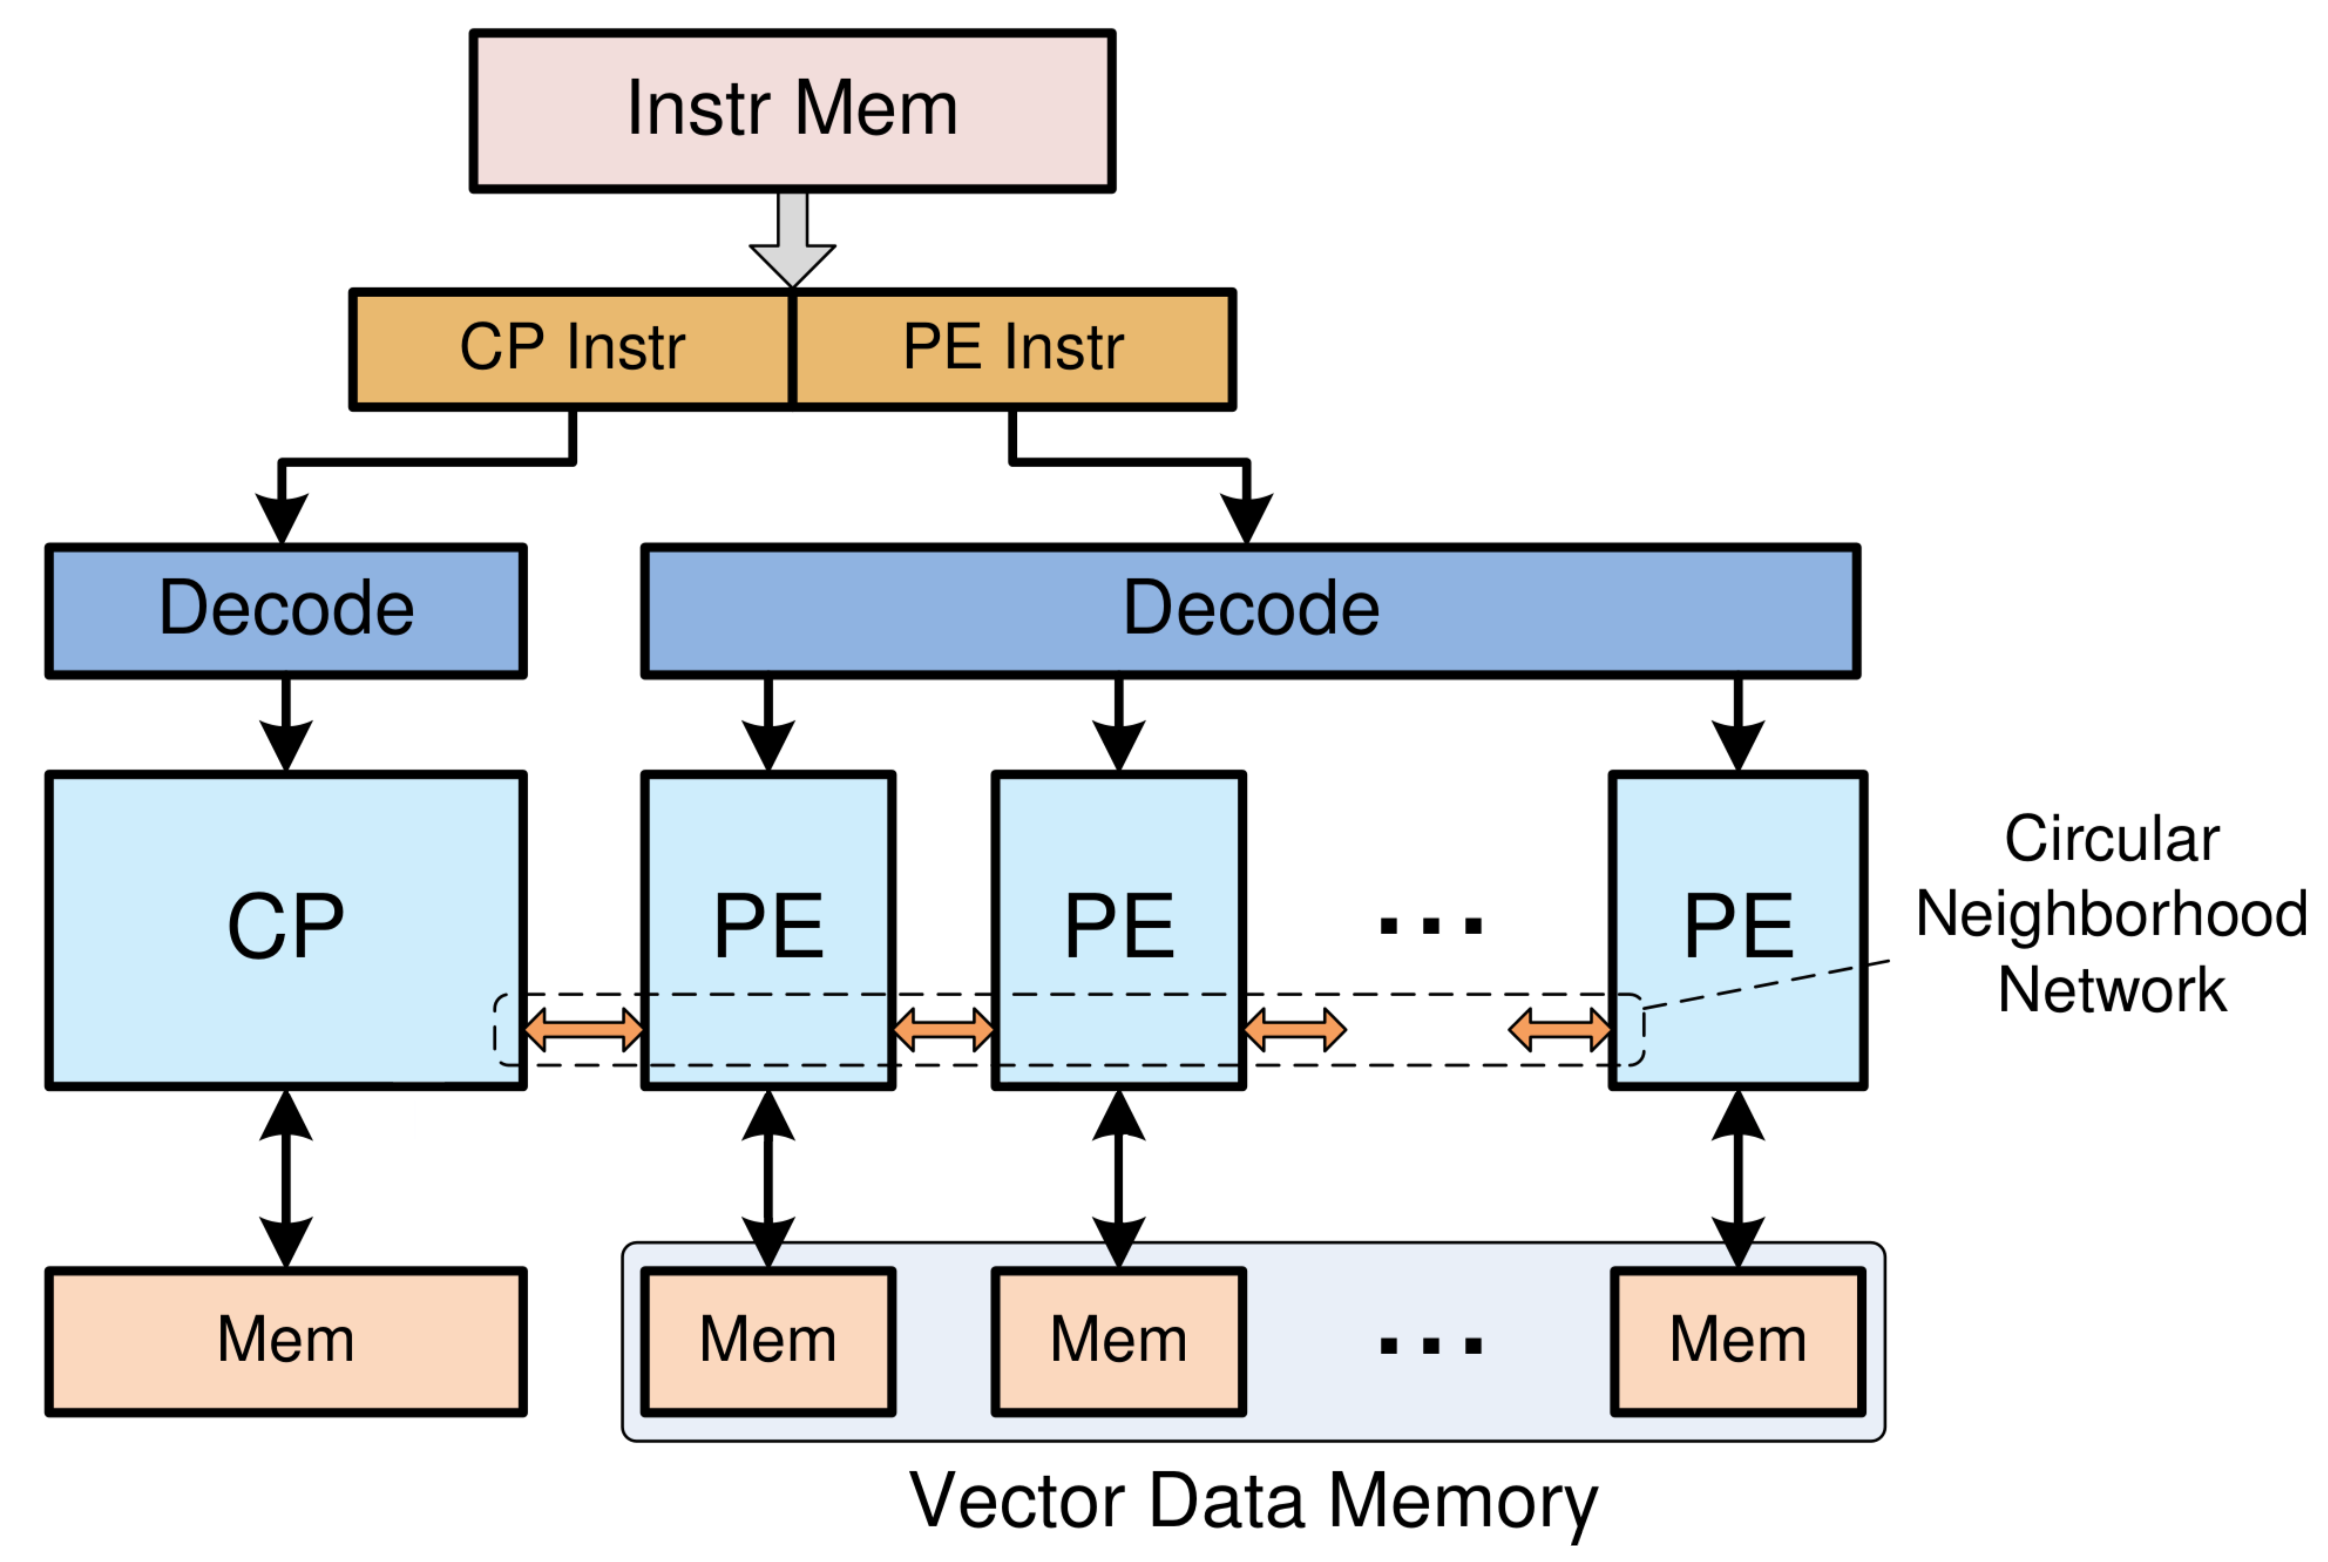
\includegraphics[width=.6\textwidth]{figures/simd_overview}
\caption{General overview of the wide SIMD architecture.}
\label{fig:simd_overview}
\end{figure}

The proposed architecture has a Reduced Instruction Set Computer (RISC) Instruction Set Architecture (ISA) that is divided up in three categories of instructions. In general, instructions have two operands and a destination register. Instructions that take two register files as operands are Register-type (R-type) instructions. Instructions that take a register file and an immediate as operands are called Immediate-type (I-type). The control flow can be controlled by using Jump-type (J-type) instructions, which can only be executed by the CP.

Furthermore, the architecture is designed to be configurable, e.g. width of the PE array, bit width of the wires and registers, the number of stages that the instruction pipeline consists of, and whether it has implicit or explicit bypassing, can be configured. The datawidth of the wires and registers can be configured into 16-bits or 32-bits.

In order to support a configurable number of PE elements, a neighbourhood network topology is chosen for its scalability. With a circular neighbourhood network topology, the connection between the first and last PE does not introduce extra long wires, because the PEs can be places in a circular manner \cite{dongrio2}.

%=============================== NN speech ===============================
%\section{Neighbourhood Network}\label{sec:nn}
%Each processor (CP or PE) does not only execute independently, but can also exchange data with its direct neighbours. However, because we have limited connectivity, moving data from one PE to another PE can introduce additional cycles. Namely, when communicating with non-direct neighbours. The circular neighbourhood network that is used to connect the processors is illustrated in Figure \ref{fig:neighborhood_network}. The CP can select data from the first and last PE, and each PE can communicate with its direct neighbours, or (not illustrated in Figure \ref{fig:neighborhood_network}) receive data from the CP by means of a broadcast.

%\begin{figure}[H]
%\centering
%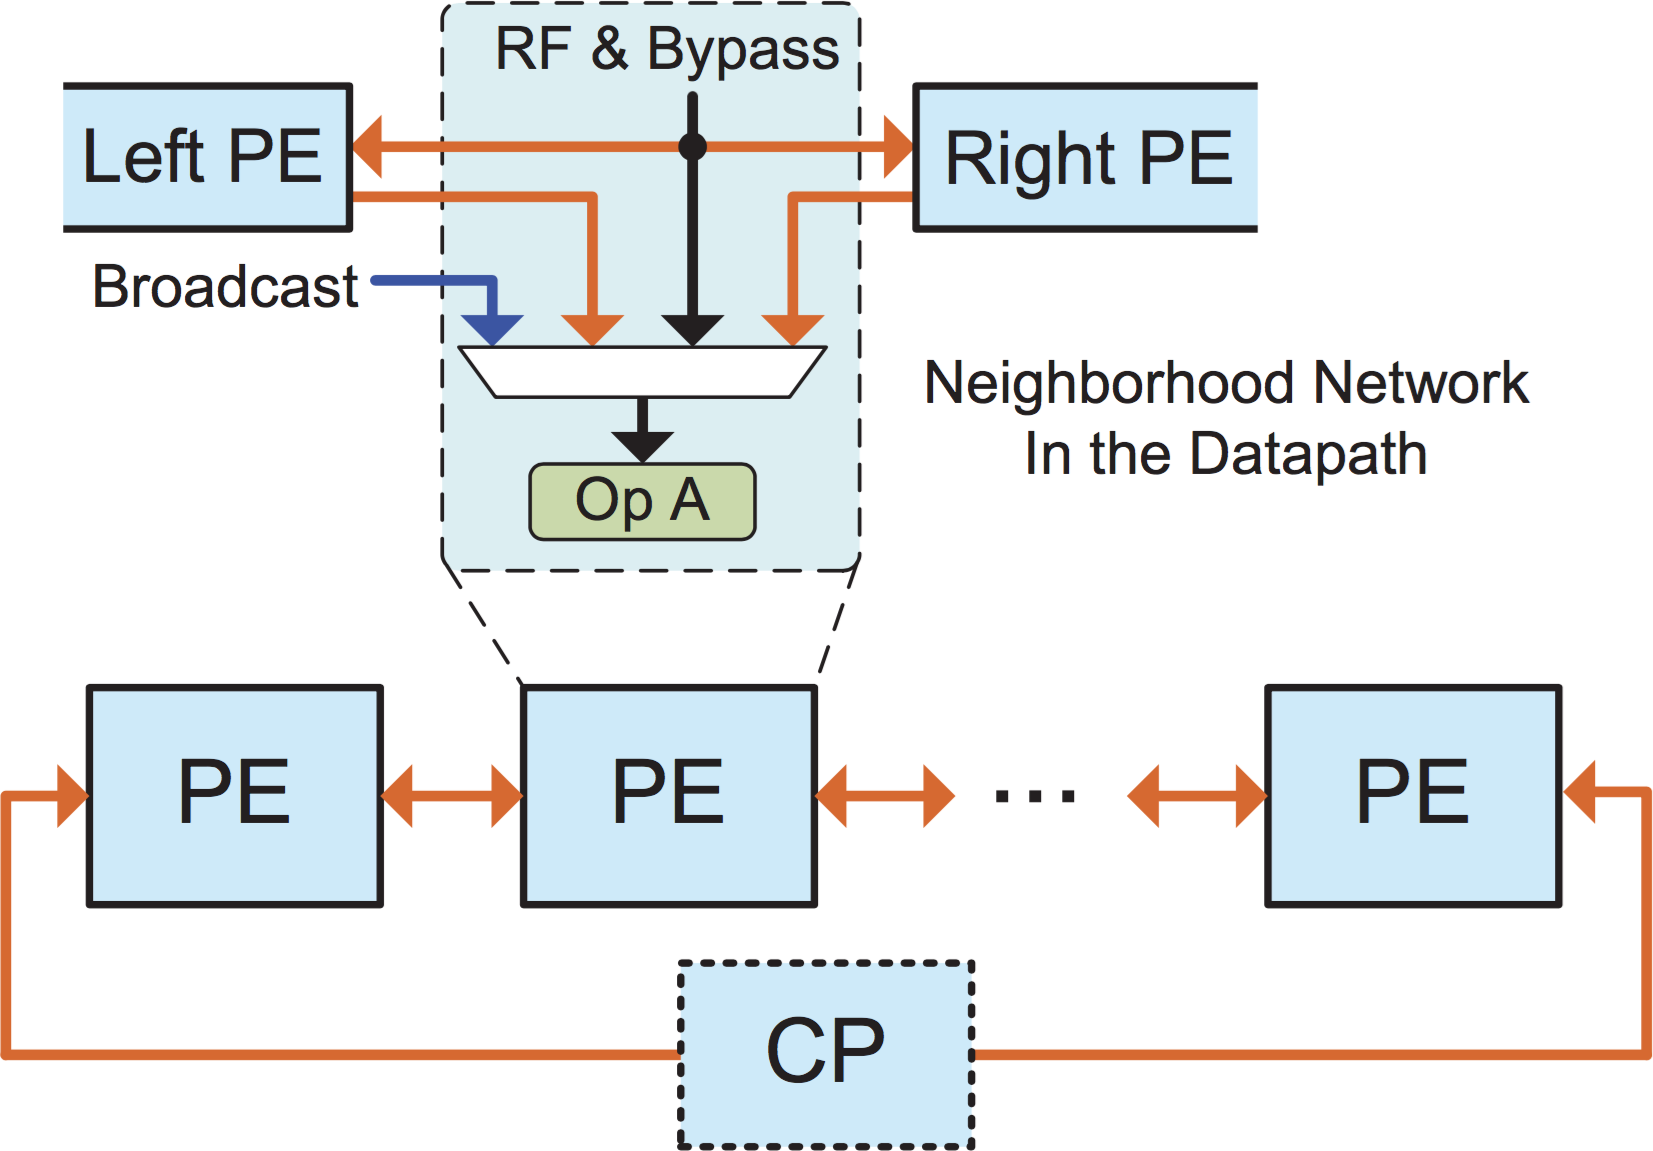
\includegraphics[width=.4\textwidth]{figures/neighborhood_network}
%\caption{Illustration of the circular neighborhood network.}
%\label{fig:neighborhood_network}
%\end{figure}

%The processor selects data from its neighbours in the instruction decode stage. Depending on the "select data" bits, it either takes data from one of its neighbours or from itself. Table \ref{table:select_data} gives an overview of the communication mode, depending on the value of "select data". The "select data" bits are decoded in each instruction, as we will show in Chapter \ref{sec:isa}.
 
% \begin{table}[H]
%\caption{Communication model for the CP and PEs, depending on the value of "select data".}
%\begin{center}
%\begin{tabular}{|c|c|c|}
%\hline
%\textbf{select data} & \textbf{CP} & \textbf{PE} \\ \hline
%2'b00 & Select data from \emph{self}. & Select data from \emph{self}. \\ \hline
%2'b01 & Select data form \emph{last} PE. & Select data from \emph{right} neighbour. \\ \hline
%2'b10 & Select data from \emph{first} PE. & Select data from \emph{left} neighbour. \\ \hline
%2'b11 & Not used. & Select data from CP \emph{broadcast}. \\ \hline
%\end{tabular}
%\end{center}
%\label{table:select_data}
%\end{table}%

%The processors communicate with each other by writing directly to the output of the operand register based on the values of bits "select data" bits. When the value of these two bits is $00$, data is selected from the processor itself. When these bits are $01$, data is selected from the last PE, in case of the CP executing this instruction, and from the right neighbour in case of a PE executing this instruction. Similarly, having a value of $10$, data is selected from the first PE in case of the CP executing this instruction, or left neighbour in case of a PE is executing this instruction. Finally, a value of $11$ will select data from the CP broadcast in the case that a PE is executing the instruction.

%=============================== Datapath speech ===============================
\subsection{Processor Pipeline and Datapath}\label{sec:processor}
%TODO: Write new paragraph about.general layout
\begin{figure}[t!]
\centering
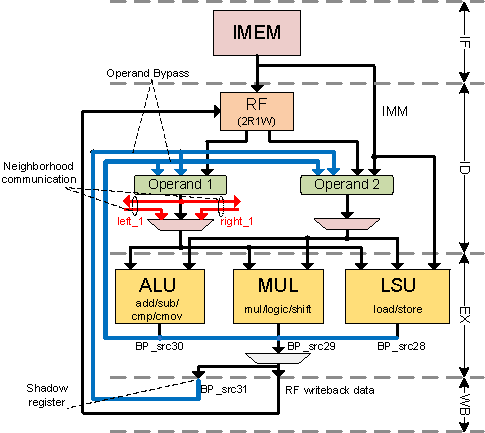
\includegraphics[width=.5\textwidth]{figures/4-stage_bypass}
\caption{4-stage pipeline processor overview.}
\label{fig:4_stage}
\end{figure}

\begin{figure}[b!]
\centering
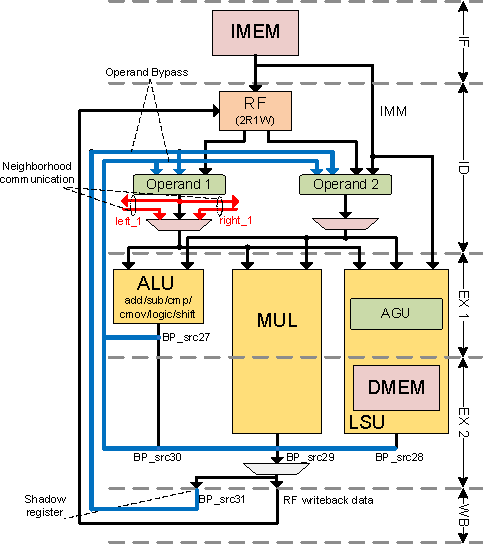
\includegraphics[width=.5\textwidth]{figures/5-stage_bypass}
\caption{5-stage pipeline with processor overview.}
\label{fig:5_stage}
\end{figure}

Generally, each processor (CP or PE) has its own registers and three functional units, i.e. ALU, MUL and LSU. 

The instruction pipeline is divided up in four or five stages. Top down, we have an IF-stage, an ID-stage, one or more execution stages and a Write Back (WB) stage. The architecture shown in Figure \ref{fig:4_stage} has four stages while the architecture shown in Figure \ref{fig:5_stage} has five stages.

The neighbourhood communication network is implemented by overriding the output of $Operand\ 1$ in ID-stage. Depending on the decoded instruction, data is either selected from another (neighbouring) processor, or from itself. Each FU has private input registers, which keep the result at the output of a compute unit valid as long as no new operation or input is assigned to it \cite{dongrio1}. The outputs can be used in the bypass network to bypass any of the operands in an instruction. 

We can configure the SIMD to have either explicit, or implicit bypassing. With implicit bypassing, also called transparent bypassing it is the hardware's responsibility to handle bypassing. With explicit bypassing on the other hand, it is the compilers responsibility to handle bypassing.

\begin{figure}[H]
\centering
\subfloat[Datapath with implicit bypassing.]{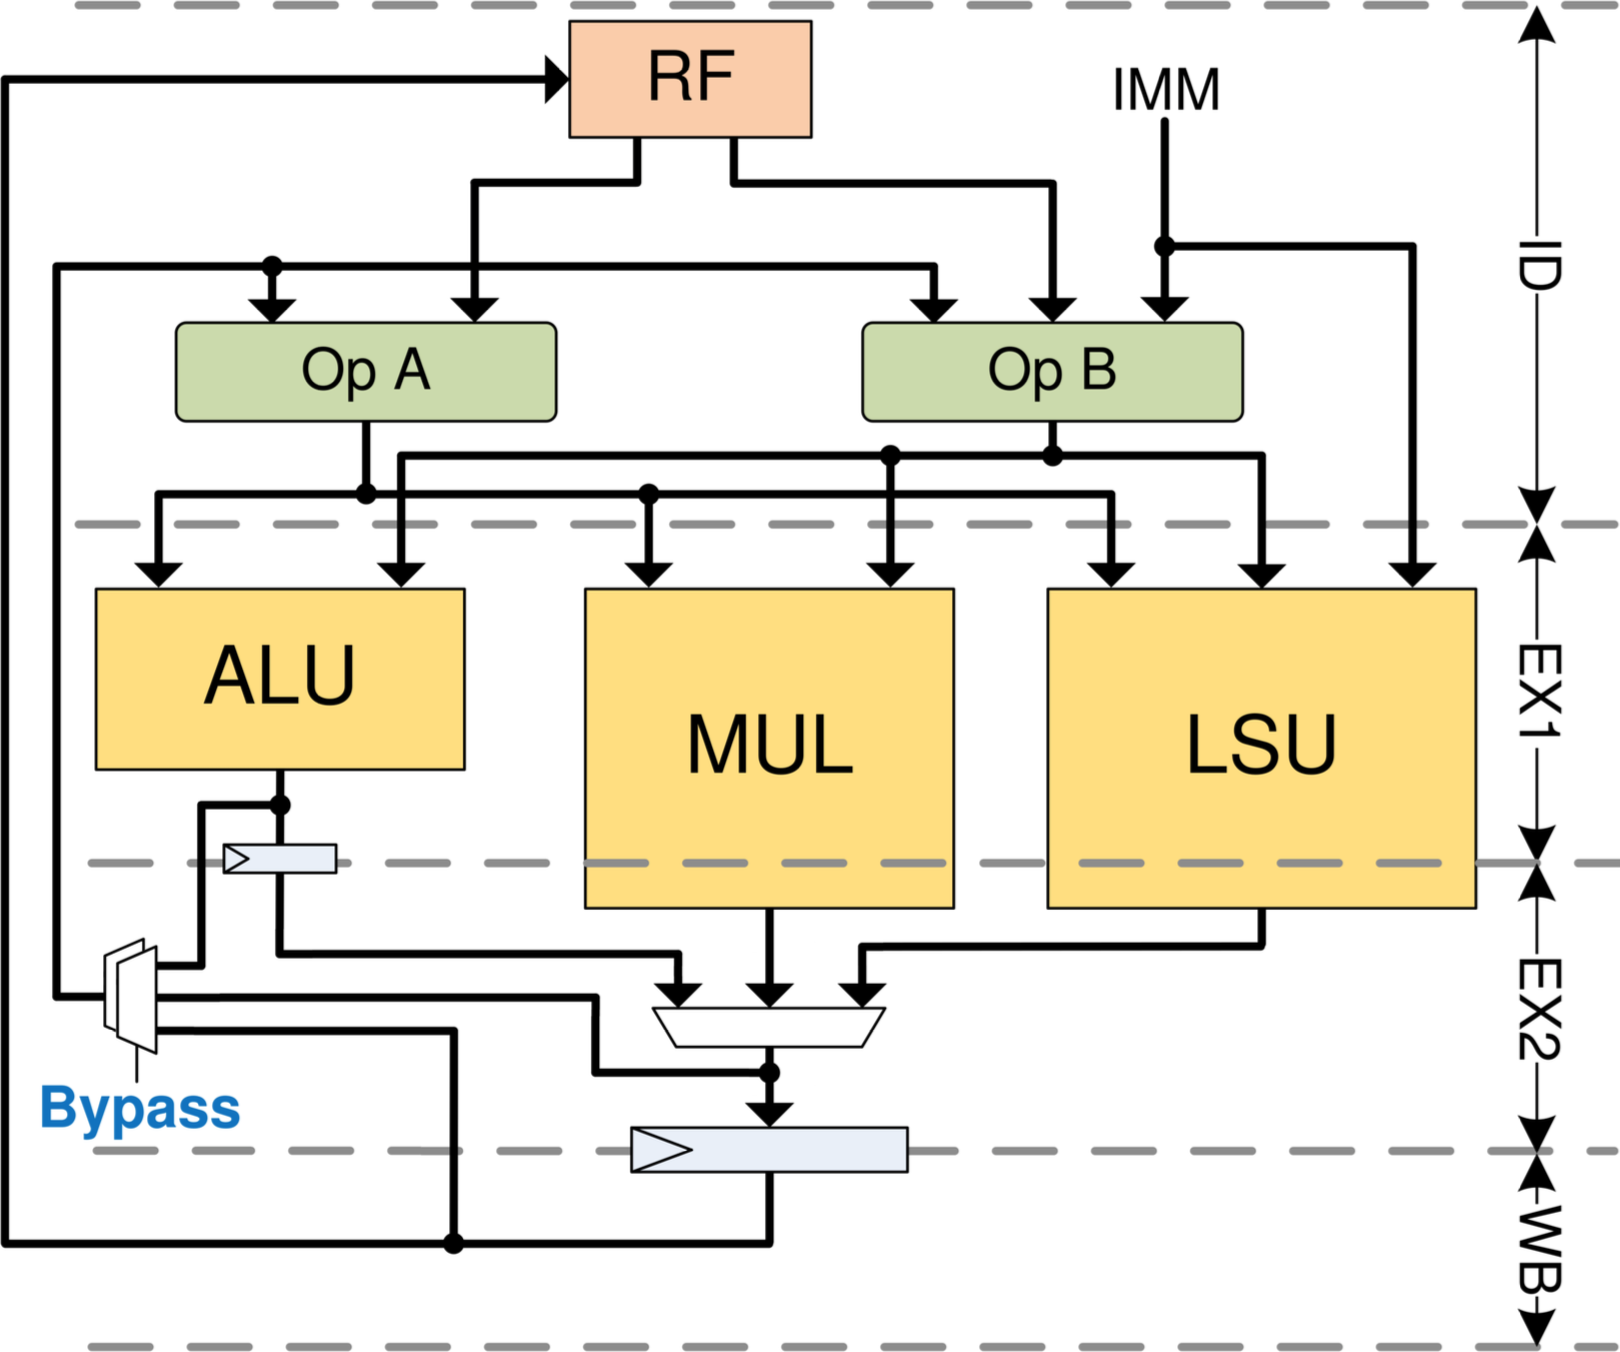
\includegraphics[width=.35\textwidth]{figures/transparent_bypass}%
\label{fig:transparent_datapath}}
\hfil
\subfloat[Datapath with explicit bypassing.]{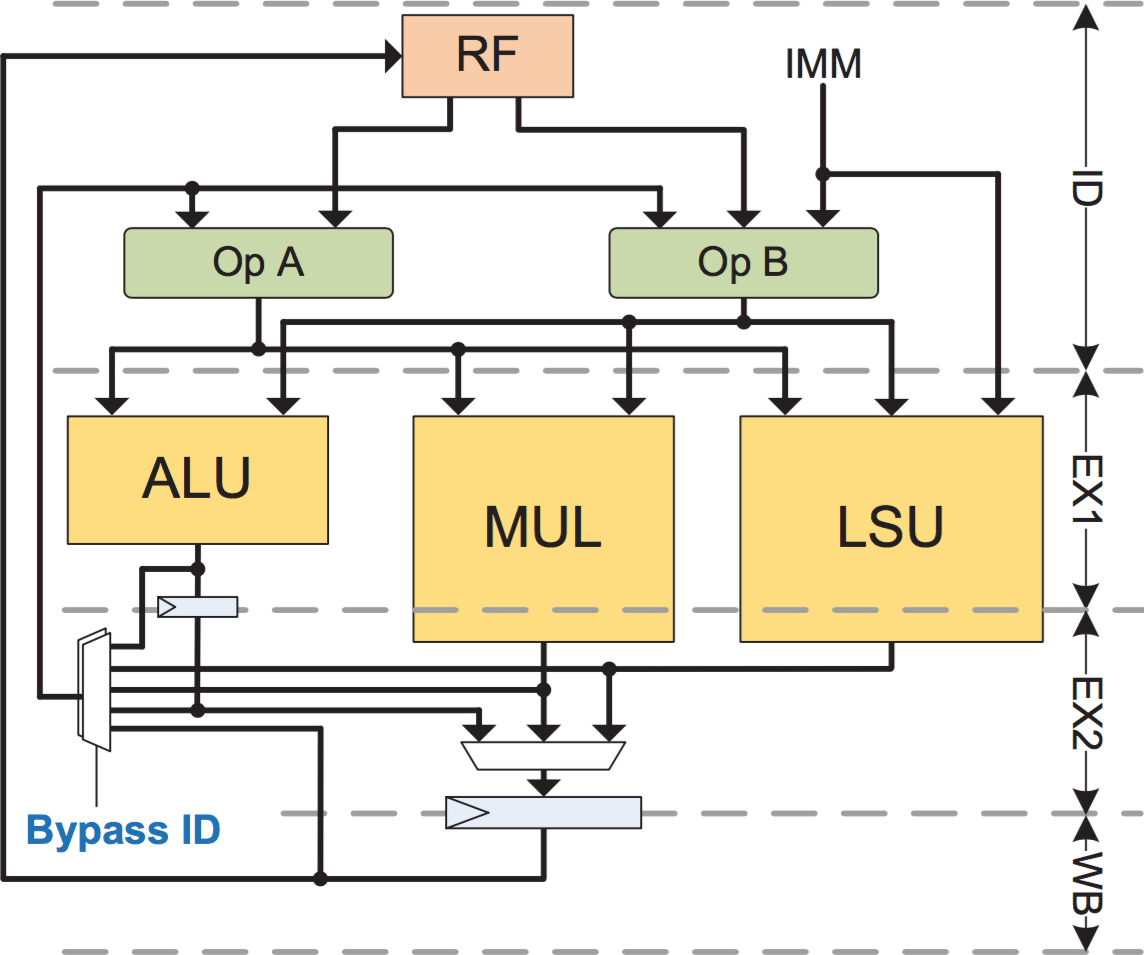
\includegraphics[width=.35\textwidth]{figures/explicit_bypass}%
\label{fig:explicit_datapath}}
\caption{Bypassing network differences between implicit bypassing and explicit bypassing.}
\label{fig:datapath_approaches}
\end{figure}

%We can configure the SIMD to have four or five stages. With four stages shown in Figure \ref{fig:4_stage}, all instructions take a single cycle, while with the five stages shown in Figure \ref{fig:5_stage}, ALU takes a single cycle, while MUL and LSU take two cycles, as shown in Table \ref{table:FU_cycles}. With 5 stages, MUL takes twice as many cycles. However, additions are simpler to perform, therefore the efficiency. 

%\begin{table}[H]
%\caption{Cycles per FU.}
%\begin{center}
%\begin{tabular}{|c|c|c|}
%\hline & \multicolumn{2}{c|}{\textbf{Cycles}} \\ \hline
%\textbf{FU} & \textbf{4-stage} & \textbf{5-stage} \\ \hline
%ALU & 1 & 1 \\ \hline
%MUL & 1 & 2 \\ \hline
%LSU & 1 & 2 \\ \hline
%\end{tabular}
%\end{center}
%\label{table:FU_cycles}
%\end{table}%

%The main difference between the two approaches is that where transparent bypassing always performs a write to a register, this is optional for explicit bypassing, as we will show in Chapter \ref{chapter:software_bypassing}.
One of the advantages of explicit bypassing is that when possible a write to a register can be avoided. Thus reducing the total energy consumption of the register file. Since there are many register files in a wide SIMD, reducing the energy consumption of the register file has a large impact on the overall energy consumption \cite{dongrio1}. Because of this, reducing the register file's energy consumption is of great importance. Furthermore, the explicit datapath shown in Figure \ref{fig:explicit_datapath} has two extra sources compared to the transparent datapath in Figure \ref{fig:transparent_datapath}. These additional bypass sources increase the chance that a result is being bypassed. In the explicit bypassing version, bypassing sources are directly accessible by the instruction. This is done by reserving part of the RF address space for the bypass sources. The disadvantage of this is that the register index space is reduced, however we do not have to change the instruction format in order to specify that an operand of an instruction is bypassed from a previous instruction.

\begin{table}[H]
\caption{Special purpose registers.}
\begin{center}
\begin{tabular}{@{}l l@{}}
\toprule
\textbf{Register} & \textbf{Purpose} \\ \hline
\emph{r0} & Constant value zero. \\
\emph{r1} & PE\_ID (PE only). \\
\emph{r3} and \emph{r4} & Return value registers. \\
\emph{r5} through \emph{r8} & Argument passing. \\
\emph{r9} & Link register (CP only). \\ 
\emph{r10} & Frame pointer. \\
\emph{r11} & Stack pointer. \\
%\multicolumn{2}{|l|}{Only with \emph{explicit bypassing}:} \\ \hline
%$R_{27}$ & $BP\_src27$ (5 stages only). \\ \hline
%$R_{28}$ & $BP\_src28$. \\ \hline
%$R_{29}$ & $BP\_src29$. \\ \hline
%$R_{30}$ & $BP\_src30$. \\ \hline
%$R_{31}$ & $BP\_src31$. \\ \hline
\bottomrule
\end{tabular}
\end{center}
\label{table:special_registers}
\end{table}%

The total number of registers grows linearly with the number of PEs because each processor has 32 registers. With a wide SIMD, we therefore have many registers that in total consume a considerable amount of energy, namely 34.6\% of the total energy consumption \cite{dongrio1}. Some of these registers have a special purpose, e.g. register $R_0$ is connected to ground is has a static value of $0$, these are shown in Table \ref{table:special_registers}.


%Todo: change this picture to have explicit and implicit bypassing instead. State then that we will be focussing on explicit bypasisng.



%Todo: add small example, having on one side normal ops. On the other hand haing implicit bypassing and finally explicit bypassing (without the store).

%\begin{figure}[b!]
%\centering
%\subfloat[4-stage pipeline with explicit datapaths.]{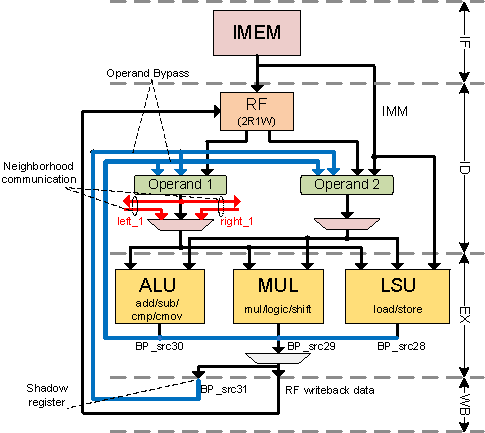
\includegraphics[width=.4\textwidth]{figures/4-stage_bypass}%
%\label{fig:4stage}}
%\hfil
%\subfloat[5-stage pipeline with explicit datapaths.]{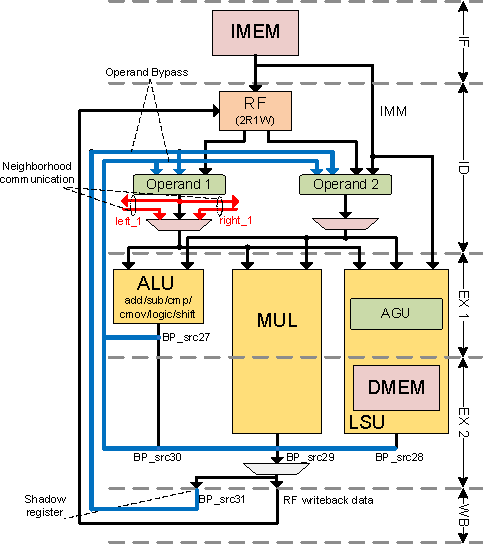
\includegraphics[width=.34\textwidth]{figures/5-stage_bypass}%
%\label{fig:5stage}}
%\caption{The pipeline of the SMD processor architecture with explicit datapaths.}
%\label{fig:pipeline_stages}
%\end{figure}

%%=============================== instruction format speech ===============================
%\section{Instruction Format}\label{sec:isa}
%%Change (optional)
%%% namely, one scalar and one vector instruction.
%%With
%%% namely, one scalar instruction that is executed on the CP, and one vector instruction that is executed on each of the PEs.
%Similar to a 2-issue VLIW instruction, an SIMD instruction consists of two subinstructions. An SIMD instruction is a 56-bit instruction that is divided up in two 28-bit subinstructions, namely, a scalar and a vector instruction. Only the CP can perform jump and branch instructions, therefore, the vector instruction can be either a R-type or an I-type instruction, while a scalar instruction can be a R-type, I-type or J-type instruction. Both sub instructions have a format, as shown in Figure \ref{fig:instruction_format}.

%\begin{figure}[H]
%\centering
%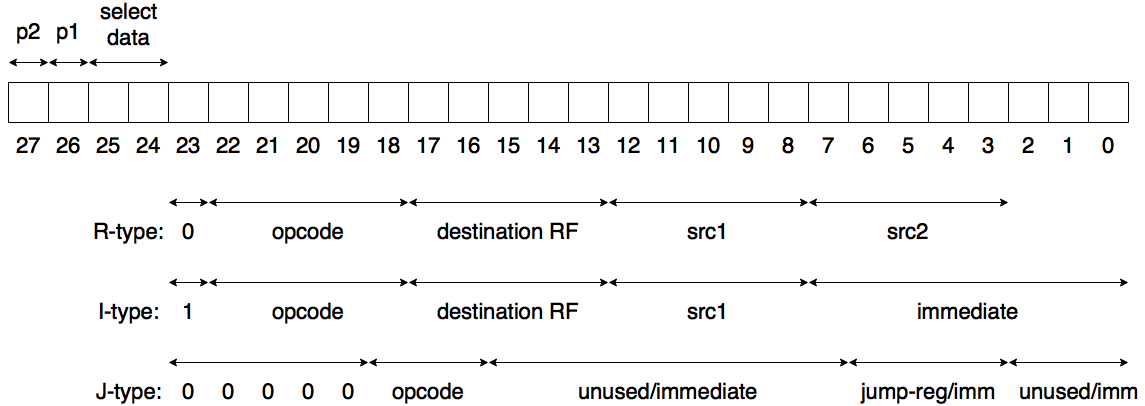
\includegraphics[width=\textwidth]{figures/instruction_format}
%\caption{Generic overview of the instruction format.}
%\label{fig:instruction_format}
%\end{figure}

%There are two guard bits $p1$ and $p2$, that can be set by using a set flag instruction. Consequently we can them for predicate execution. The instructions, branch if flag (not) set and conditional move read the predicate flag before executing. For the full overview of supported instructions, see Appendix \ref{chapter:supported_operations}.

%Note that the "select data" bits are also part of the instruction as we explained in Chapter \ref{sec:nn}. The CP and PEs can communicate by setting these bits. The communication model is shown in Table \ref{table:select_data}.


\section{The LLVM Compiler Framework}\label{sec:llvm}
The LLVM project started in 2000 by Chris Lattner, as a research project at the University of Illinois with the goal of providing a modern, Static Single Assignment (SSA)-based compilation strategy capable of supporting both static and dynamic compilation of arbitrary programming languages. It was first released in 2003, although the project has grown rapidly since then. It has become popular amongst major companies, e.g. Google, Apple and Sony, for its powerful multi-stage compilation strategy and outstanding extendibility. LLVM is a collection of modular and reusable compiler and toolchain technologies. Generally, LLVM follows a 3-phase design, which is divided up in a frontend, a code independent optimizer and a backend, illustrated in Figure \ref{fig:3phase_design}.

\begin{figure}[H]
\centering

\includegraphics[width=.7\textwidth]{figures/3phase_design}
\caption{3-phase design: frontend, optimizer and backend.}
\label{fig:3phase_design}
\end{figure}

%Reorder list: [IR, Lexical analysis, Syntax analysis, ]
\textbf{The frontend} is responsible for translating code of an arbitrary language into LLVM's Intermediate Representation (IR) code. The LLVM instruction set represents a virtual architecture that captures the key operations of ordinary processors, but avoids machine specific constraints such as physical registers. Instead, it has an infinite amount of virtual registers in SSA form, which means that each virtual register is assigned only once and each use of a variable is dominated by that variable's definition. This simplifies the dataflow optimizations because only a single definition can reach a particular use of a value, and finding that definition is trivial \cite{llvm_strategy}.
%frontend talk, straight from the Dragon Book plz.
%introduce parser and lexical analysis and that it is kept in an AST, which will be translated as a final step to IR.
%Perhaps an example?
%TODO: rewrite first sentence in my own words.
As the first phase of a compiler, the main task of the lexical analyzer is to read the input characters of the source program, group them into luxemes, and produce as output a sequence of tokens. These tokens are used by the parser for syntax analysis, where we verify that the sequence of tokens can be reconstructed according to the syntax of the input language. The parser should report any syntax errors during this process and should be able to recover in order to continue processing the rest of the program. The parser constructs a parse tree, and the semantic analyzer uses this parse tree to check for consistency with the language definition. Type checking is also done during this stage, and the information is kept in the syntax tree. The result of these phases is an Abstract Synctax Tree (AST) of the program, which can be translated into three-address IR code. %We will discuss LLVM's IR in more detail in Chapter \ref{sec:ir}

\textbf{The optimizer} contains a collections of analysis and semantic-preserving transformations that can be used to optimize IR code. One of the advantages of LLVM is that when you build a new backend for any given processor architecture you immediately have access to all of these optimizations. Below we give some of these optimizations that are explained more detailed in literature \cite[Chapter~9]{dragon_book}.%TODO: provide chapter in cite.
\begin{itemize}
\item \emph{Constant propagation} computes for each point and each variable in the program, whether that variable has a unique constant value at that point. This can then be used to replace variable references with constant values.
\item \emph{Constant folding} recognizes and evaluates constant expressions at compile time rather than runtime. For example, `$add\ 1+2$' can be replaced by `$3$'. Statements like `$add\ 1+2$' can be introduced by other optimizations, e.g. constant propagation. 
\item \emph{Common sub-expression elimination} recognizes that the same expressions appears in more than one place, and that performance can be improved by transforming the code such that the expression appears in one only place.
\item \emph{Copy propagation} replaces each target of a copy statement with that of the copied value. For example, if we have a copy statement, $x = y$. Then the uses of $x$ can be replaced by $y$. Some optimizations require that this optimizations is performed afterwards to cleanup, e.g. common sub-expression elimination requires this pass to run afterwards. 
\item \emph{Dead code elimination} removes code that do not affect the programs results. This avoids executing irrelevant operations and reduces the code size of a program.  
\item \emph{Loop invariant code motion} aims at moving code that is independent of the loop iteration out of the loop body. It does this by moving the loop independent statement above the loop, saving it in a temporary variable, and use it in each iteration of the loop. Now the loop independent statement is computed only once instead of every iteration. 
\item \emph{Function inlining} verifies whether inlining functions in its callees gives a performance benefit. If doing this would give performance benefit, it replaces the call of the function with the function body. This optimization often is useful for small functions because it reduces the overhead that is introduced when a function call is made, e.g. storing frame pointer, storing function parameters and jump in code to where the function is defined.     
\end{itemize}

\begin{figure}[b!]
\centering
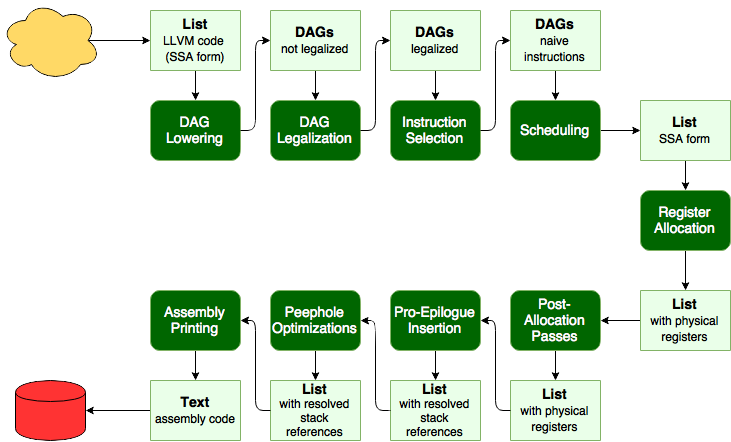
\includegraphics[width=\textwidth]{figures/code_generation_sequence}
\caption{Code generation sequence, from LLVM code to assembly code.}
\label{fig:code_generation}
\end{figure}

%TODO: apply following namings: Instruction, Machine instruction, scheduled instruction in SSA form, schedule instruction not in SSA form.
\textbf{The backend} translates, according to a processor architecture, IR code to a target specific assembly language. It does this by going through a sequence of code generation stages, illustrated in Figure \ref{fig:code_generation}. The rectangular boxes indicate the data structure that is used by, and produced by a given stage, and the name of each stage is denoted in a rectangular box with rounded corners. During this process, first the IR code is lowered to a Directed Acyclic Graph (DAG) in which each node represents one instruction. However, for some architectures, not all data types and instructions are supported. For this reason, the DAG is legalized to something that is supported by the target architecture. Instruction selection maps each of the nodes into machine nodes, by matching patterns. %After that, the instruction selector maps the pattern of LLVM code into the target machine code and builds a new DAG whose nodes represents the target instructions.
Then we have a DAG consisting of only target specific machine instructions, in SSA form. Having naive machine instruction, the next step is to schedule them. We schedule the machine instructions according to the resource information of the target processor, and assign each instruction to a specific cycle. 
%We will discuss scheduling in more detail in Chapter \ref{sec:scheduling}. 
Now the instructions are represented in a list rather than a DAG, but still in SSA form. The Register Allocator (RA) then assigns physical registers to each of the virtual registers, now the list is not in SSA form. 
%We will discuss RA in more detail in Chapter \ref{sec:register_allocation}. 
The post-allocation pass can improve the schedule, taking the physical registers and register pressure, that is known at this point, into account. After that, some epilogue and prologue code might need to be inserted, e.g. saving/restoring the caller/callee registers and reserving/destroying of the function's stack frame. The peephole optimizations are target specific improvements to the schedule that has been constructed. These optimizations deal with very specific optimizations that can only be done at the end of the process. At last, the assembly printer, prints the assembly code.
%backend talk -> huuge



%\subsection{Instruction Scheduling}\label{sec:scheduling}
%After instruction selection, the program is represented in SSA form as a DAG. Each instruction is represented as a $MachineSDNode$ in a $MachineBasicBlock$. After scheduling has been performed, each instructions now is represented as a $MachineInstr$. 



%ach instruction is scheduleDuring instruction schdduling, each $MachineBasicBlock$ is scheduled by the scheduler and transformed into a $MachineInstr$. After this phase, instructions are represented as $MachineInstr$.

%\subsection{Register Allocation}\label{sec:register_allocation}
%Register allocation is executed during the code generation phase and consists of finding a mapping of a program with an unlimited number of virtual registers to a program with a limited number of physical registers.
%Examples, machine instrs on the left in SSA form, on the right with proper registers next to it.
%Introduce at least 

\subsection{Scheduling and RA}
TODO: exlain phase ordering between scheduling and RA, from ref \cite[Chapter~10.2.4]{dragon_book}.

Introduce terms spilling, register pressure, and use this reference \cite{ra}.




%Additional ref. 
%






%Problem statement -> incorporate Roel's Feedback..!!!
\section{Problem statement}\label{sec:problem_statement}
An SIMD architecture has been designed and a legacy compiler exists. However, the legacy compiler is too custom and therefore difficult to maintain. Many optimizations still have to be implemented. One of the advantages of LLVM is that a large community works on it. Many optimizations are already in place and can immediately be used for our compiler. Standardizing and having proper tool support improves maintainability of the compiler. %Namely, anyone familiar with LLVM can now understand and improve the compiler.
For this reason, a new compiler is being implemented in LLVM.

We have a new compiler in LLVM that supports vector operations and can compile any IR code into SIMD specific assembly. The legacy compiler does have support for explicit bypassing. We want to develop explicit bypassing in the new compiler structure.

The goal of this project is therefore to generate efficient code to support explicit bypassing. We have separated the goal in multiple research questions:

\begin{enumerate}
\item How do we implement explicit bypassing within LLVM?

How does this fit in the new compiler.
\item What alternative approaches are there to implement it?

Do we do this in an early stage, or at a later stage in the compiler.
\item How do we know which approach is more efficient?

What metric would be suitable to evaluate the different approaches with each other and with the legacy compiler.
\end{enumerate}



%Deelvragen:
% - Hoe impl. ik expl. in LLVM
% - Wat zijn de stappen
% - Alternatieven aanpakken
% - Hoe weet ik welke beter is
% - Hoe is dat nuttig voor andere architecture


%Overview
\section{Overview}\label{sec:overview}
In the remainder of this report we will discuss related works in Chapter \ref{chapter:related_work}. We will discuss bypassing, and show the difference between implicit and explicit bypassing in Chapter \ref{chapter:explicit_bypassing}. Proposed solutions for how to achieve our goal will be discussed in Chapter \ref{chapter:solutions}. We will provide a planning for this master thesis in Chapter \ref{chapter:planning} and early conclusions are given in Section \ref{chapter:conclusions}.

%\clearemptydoublepage

%\chapter{Preliminaries}\label{chapter:preliminaries}
%This template has been used to publish the thesis of Buijs~\cite{MScBuijs2010} and is originally used for the thesis of Nugteren~\cite{MScNugteren2010}. 

One of the best resources for \LaTeX basics, and advanced constructs, is the \LaTeX wikibook\footnote{To be found at~\url{http://en.wikibooks.org/wiki/LaTeX/}}. Of course colleagues and a good internet search using your favorite search engine can do wonders if you're stuck. 

%\clearemptydoublepage

%\chapter{The SIMD Processor Architecture}\label{chapter:simd}
%The advantage of the SIMD architecture is that multiple operations are processed in parallel instead of processing them in a sequence. Therefore, the same performance can be achieved at a much lower clock frequency, thereby reducing energy consumption \cite{dongrio1}. Furthermore, because each Processing Element (PE) executes the same instruction, the Instruction Fetch (IF) and Instruction Decode (ID) can be shared amongst the PEs, reducing energy consumption.

We propose a wide SIMD architecture \cite{simd} that performs wide vector operations that exploit DLP by executing the same instruction on multiple data simultaneously. Figure \ref{fig:simd_overview} shows a general overview of the SIMD processor.
We have one Control Processor (CP) responsible for scalar operations and control flow e.g. jump/branch instruction. Furthermore there is a wide array of PEs responsible for vector operations. The CP executes in parallel with the PEs, exploiting ILP.

\begin{figure}[H]
\centering
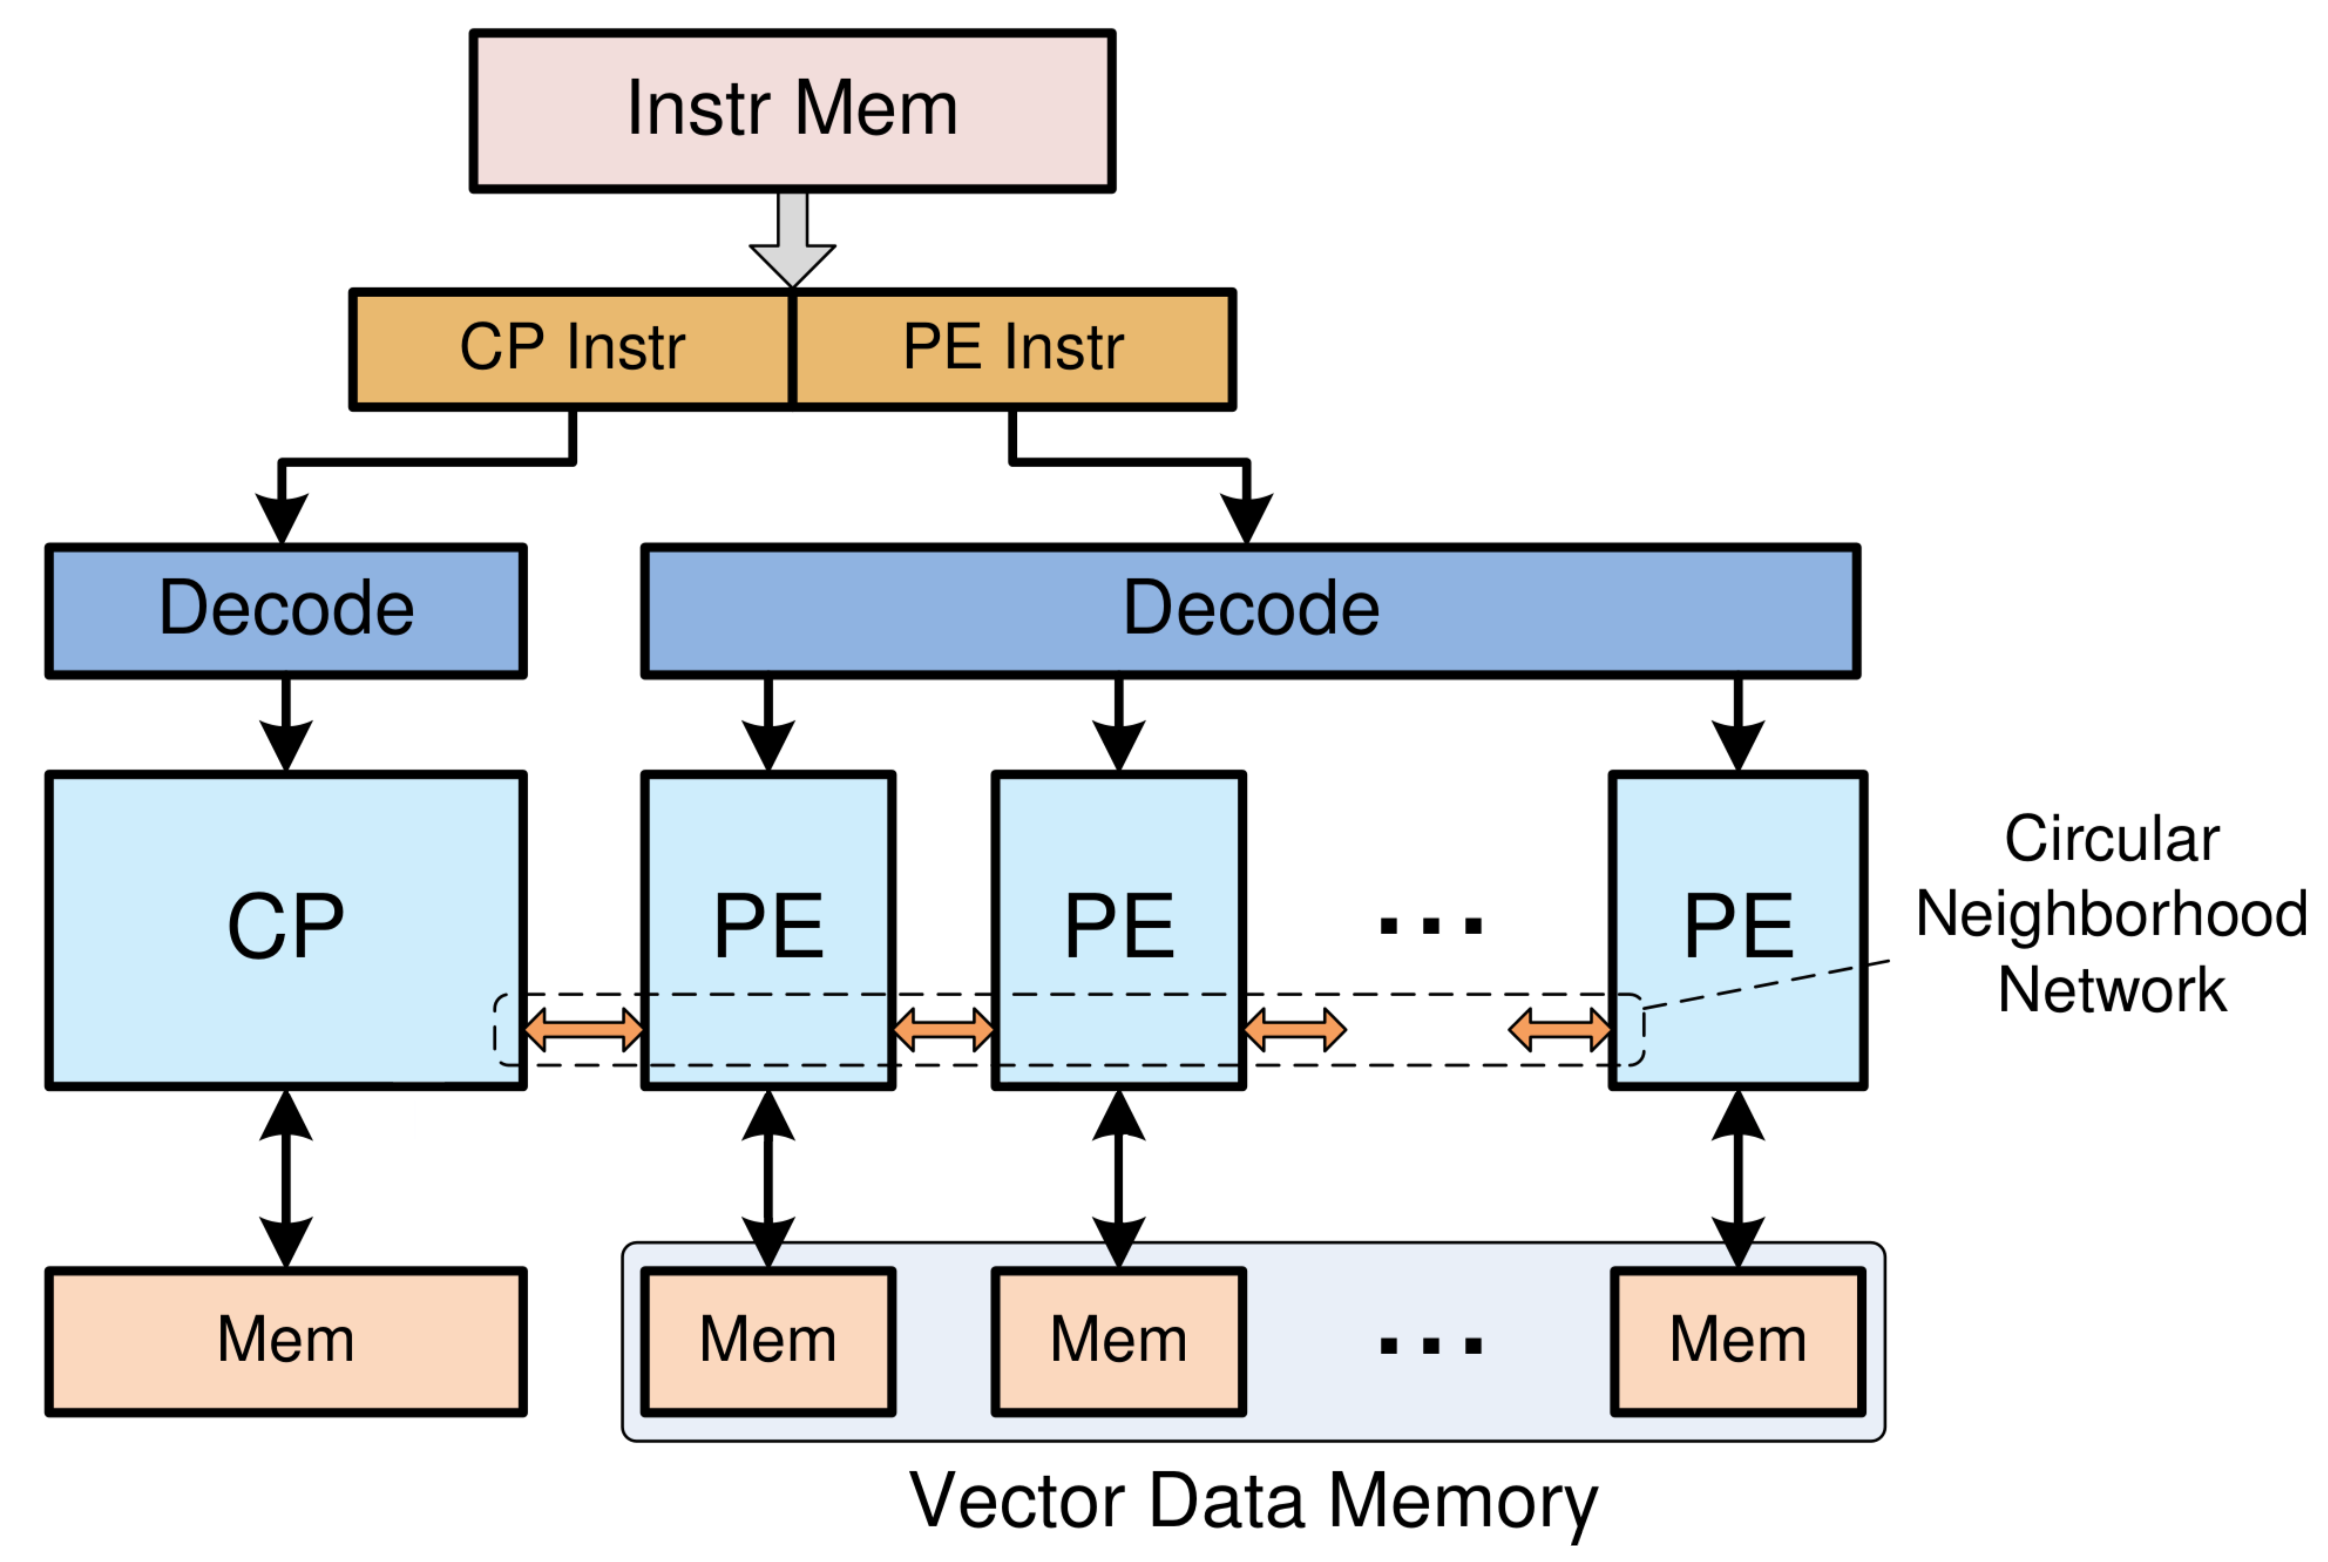
\includegraphics[width=.6\textwidth]{figures/simd_overview}
\caption{General overview of the wide SIMD architecture.}
\label{fig:simd_overview}
\end{figure}

The proposed architecture has a Reduced Instruction Set Computer (RISC) Instruction Set Architecture (ISA) that is divided up in three categories of instructions. In general, instructions have two operands and a destination register. Instructions that take two register files as operands are Register-type (R-type) instructions. Instructions that take a register file and an immediate as operands are called Immediate-type (I-type). The control flow can be controlled by using Jump-type (J-type) instructions, which can only be executed by the CP.

Furthermore, the architecture is designed to be configurable, e.g. width of the PE array, bit width of the wires and registers, the number of stages that the instruction pipeline consists of, and whether it has implicit or explicit bypassing, can be configured. The datawidth of the wires and registers can be configured into 16-bits or 32-bits.

In order to support a configurable number of PE elements, a neighbourhood network topology is chosen for its scalability. With a circular neighbourhood network topology, the connection between the first and last PE does not introduce extra long wires, because the PEs can be places in a circular manner \cite{dongrio2}.

%=============================== NN speech ===============================
%\section{Neighbourhood Network}\label{sec:nn}
%Each processor (CP or PE) does not only execute independently, but can also exchange data with its direct neighbours. However, because we have limited connectivity, moving data from one PE to another PE can introduce additional cycles. Namely, when communicating with non-direct neighbours. The circular neighbourhood network that is used to connect the processors is illustrated in Figure \ref{fig:neighborhood_network}. The CP can select data from the first and last PE, and each PE can communicate with its direct neighbours, or (not illustrated in Figure \ref{fig:neighborhood_network}) receive data from the CP by means of a broadcast.

%\begin{figure}[H]
%\centering
%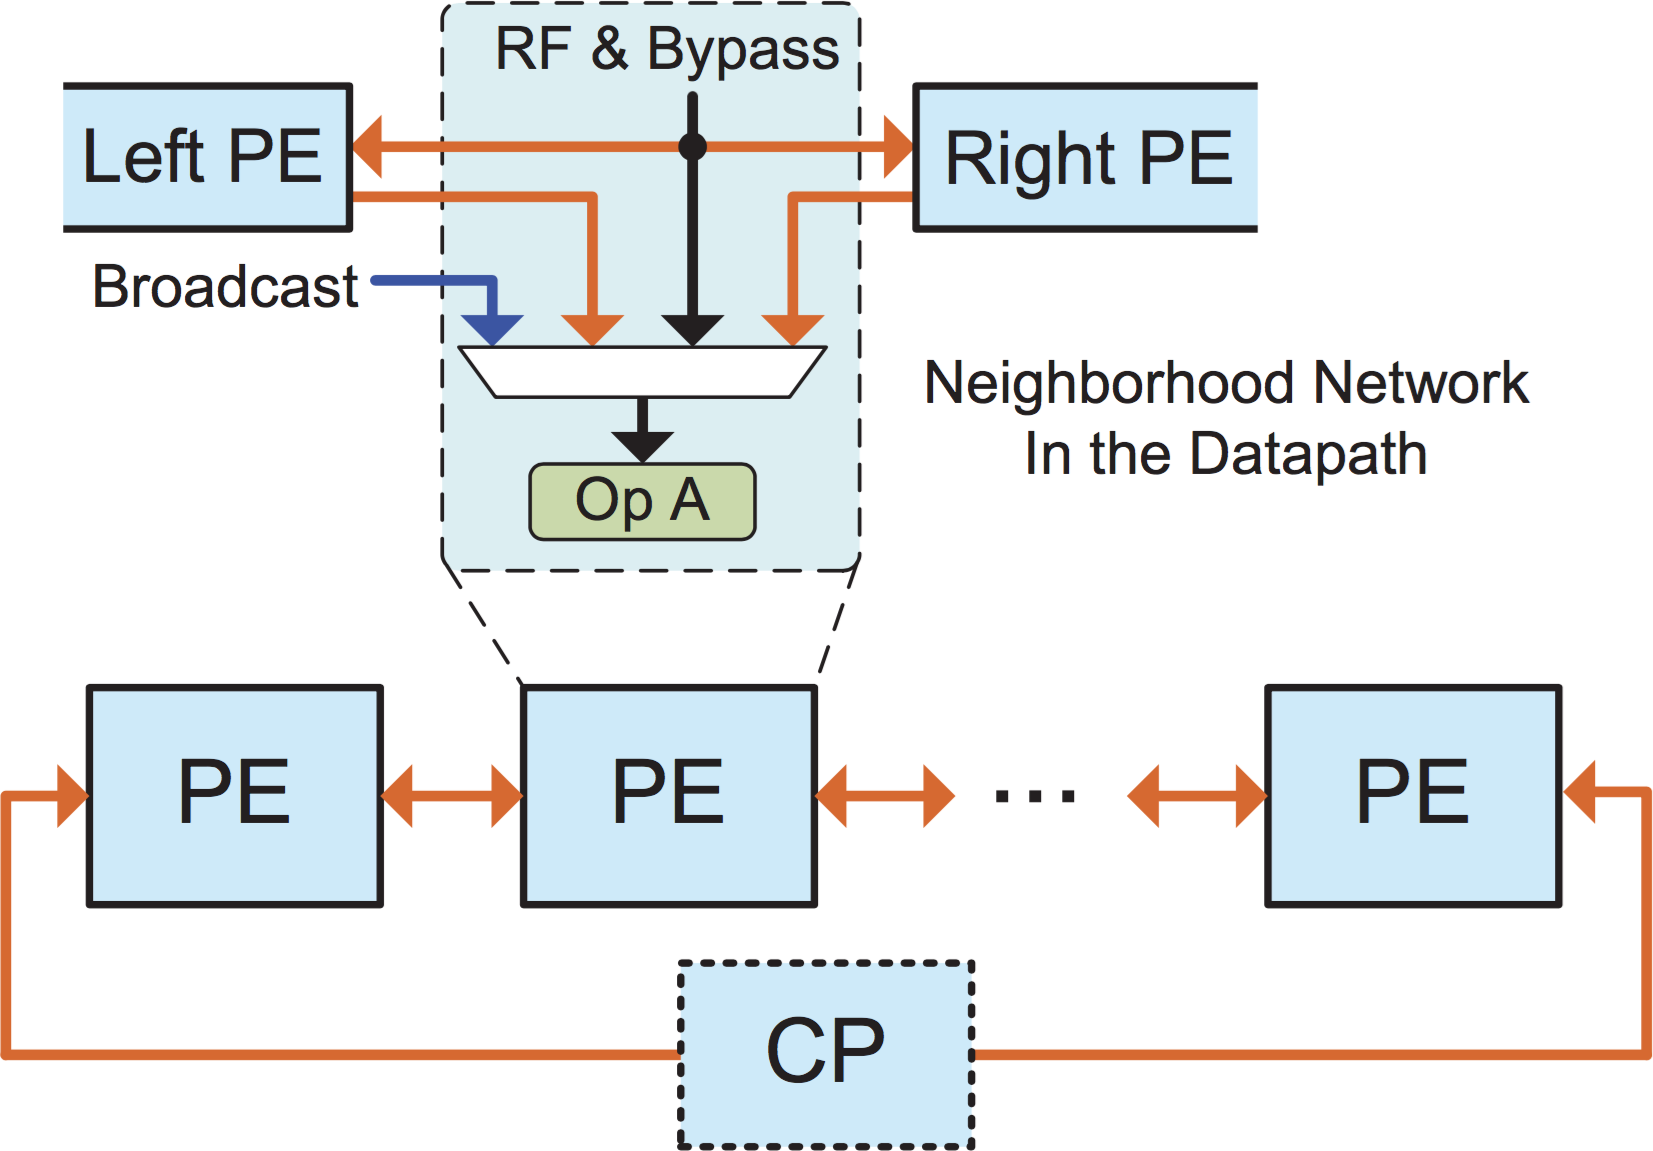
\includegraphics[width=.4\textwidth]{figures/neighborhood_network}
%\caption{Illustration of the circular neighborhood network.}
%\label{fig:neighborhood_network}
%\end{figure}

%The processor selects data from its neighbours in the instruction decode stage. Depending on the "select data" bits, it either takes data from one of its neighbours or from itself. Table \ref{table:select_data} gives an overview of the communication mode, depending on the value of "select data". The "select data" bits are decoded in each instruction, as we will show in Chapter \ref{sec:isa}.
 
% \begin{table}[H]
%\caption{Communication model for the CP and PEs, depending on the value of "select data".}
%\begin{center}
%\begin{tabular}{|c|c|c|}
%\hline
%\textbf{select data} & \textbf{CP} & \textbf{PE} \\ \hline
%2'b00 & Select data from \emph{self}. & Select data from \emph{self}. \\ \hline
%2'b01 & Select data form \emph{last} PE. & Select data from \emph{right} neighbour. \\ \hline
%2'b10 & Select data from \emph{first} PE. & Select data from \emph{left} neighbour. \\ \hline
%2'b11 & Not used. & Select data from CP \emph{broadcast}. \\ \hline
%\end{tabular}
%\end{center}
%\label{table:select_data}
%\end{table}%

%The processors communicate with each other by writing directly to the output of the operand register based on the values of bits "select data" bits. When the value of these two bits is $00$, data is selected from the processor itself. When these bits are $01$, data is selected from the last PE, in case of the CP executing this instruction, and from the right neighbour in case of a PE executing this instruction. Similarly, having a value of $10$, data is selected from the first PE in case of the CP executing this instruction, or left neighbour in case of a PE is executing this instruction. Finally, a value of $11$ will select data from the CP broadcast in the case that a PE is executing the instruction.

%=============================== Datapath speech ===============================
\subsection{Processor Pipeline and Datapath}\label{sec:processor}
%TODO: Write new paragraph about.general layout
\begin{figure}[t!]
\centering
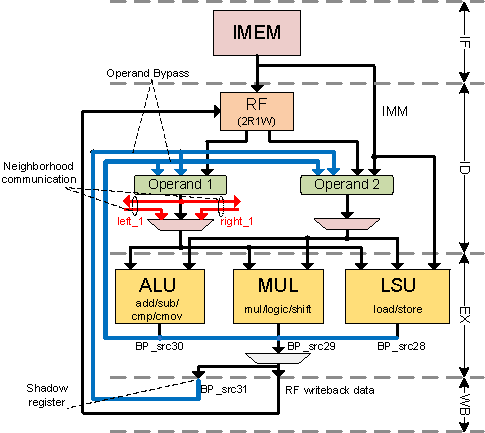
\includegraphics[width=.5\textwidth]{figures/4-stage_bypass}
\caption{4-stage pipeline processor overview.}
\label{fig:4_stage}
\end{figure}

\begin{figure}[b!]
\centering
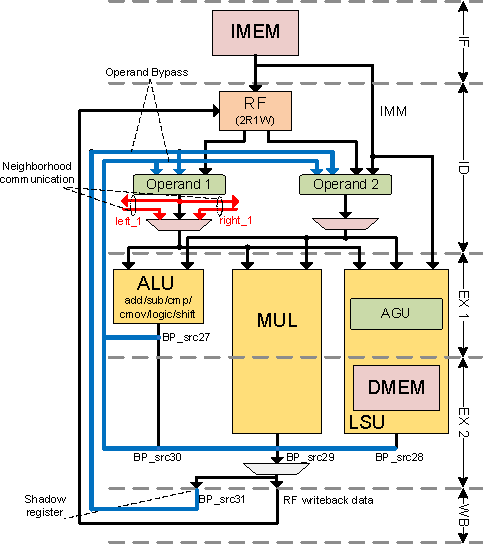
\includegraphics[width=.5\textwidth]{figures/5-stage_bypass}
\caption{5-stage pipeline with processor overview.}
\label{fig:5_stage}
\end{figure}

Generally, each processor (CP or PE) has its own registers and three functional units, i.e. ALU, MUL and LSU. 

The instruction pipeline is divided up in four or five stages. Top down, we have an IF-stage, an ID-stage, one or more execution stages and a Write Back (WB) stage. The architecture shown in Figure \ref{fig:4_stage} has four stages while the architecture shown in Figure \ref{fig:5_stage} has five stages.

The neighbourhood communication network is implemented by overriding the output of $Operand\ 1$ in ID-stage. Depending on the decoded instruction, data is either selected from another (neighbouring) processor, or from itself. Each FU has private input registers, which keep the result at the output of a compute unit valid as long as no new operation or input is assigned to it \cite{dongrio1}. The outputs can be used in the bypass network to bypass any of the operands in an instruction. 

We can configure the SIMD to have either explicit, or implicit bypassing. With implicit bypassing, also called transparent bypassing it is the hardware's responsibility to handle bypassing. With explicit bypassing on the other hand, it is the compilers responsibility to handle bypassing.

\begin{figure}[H]
\centering
\subfloat[Datapath with implicit bypassing.]{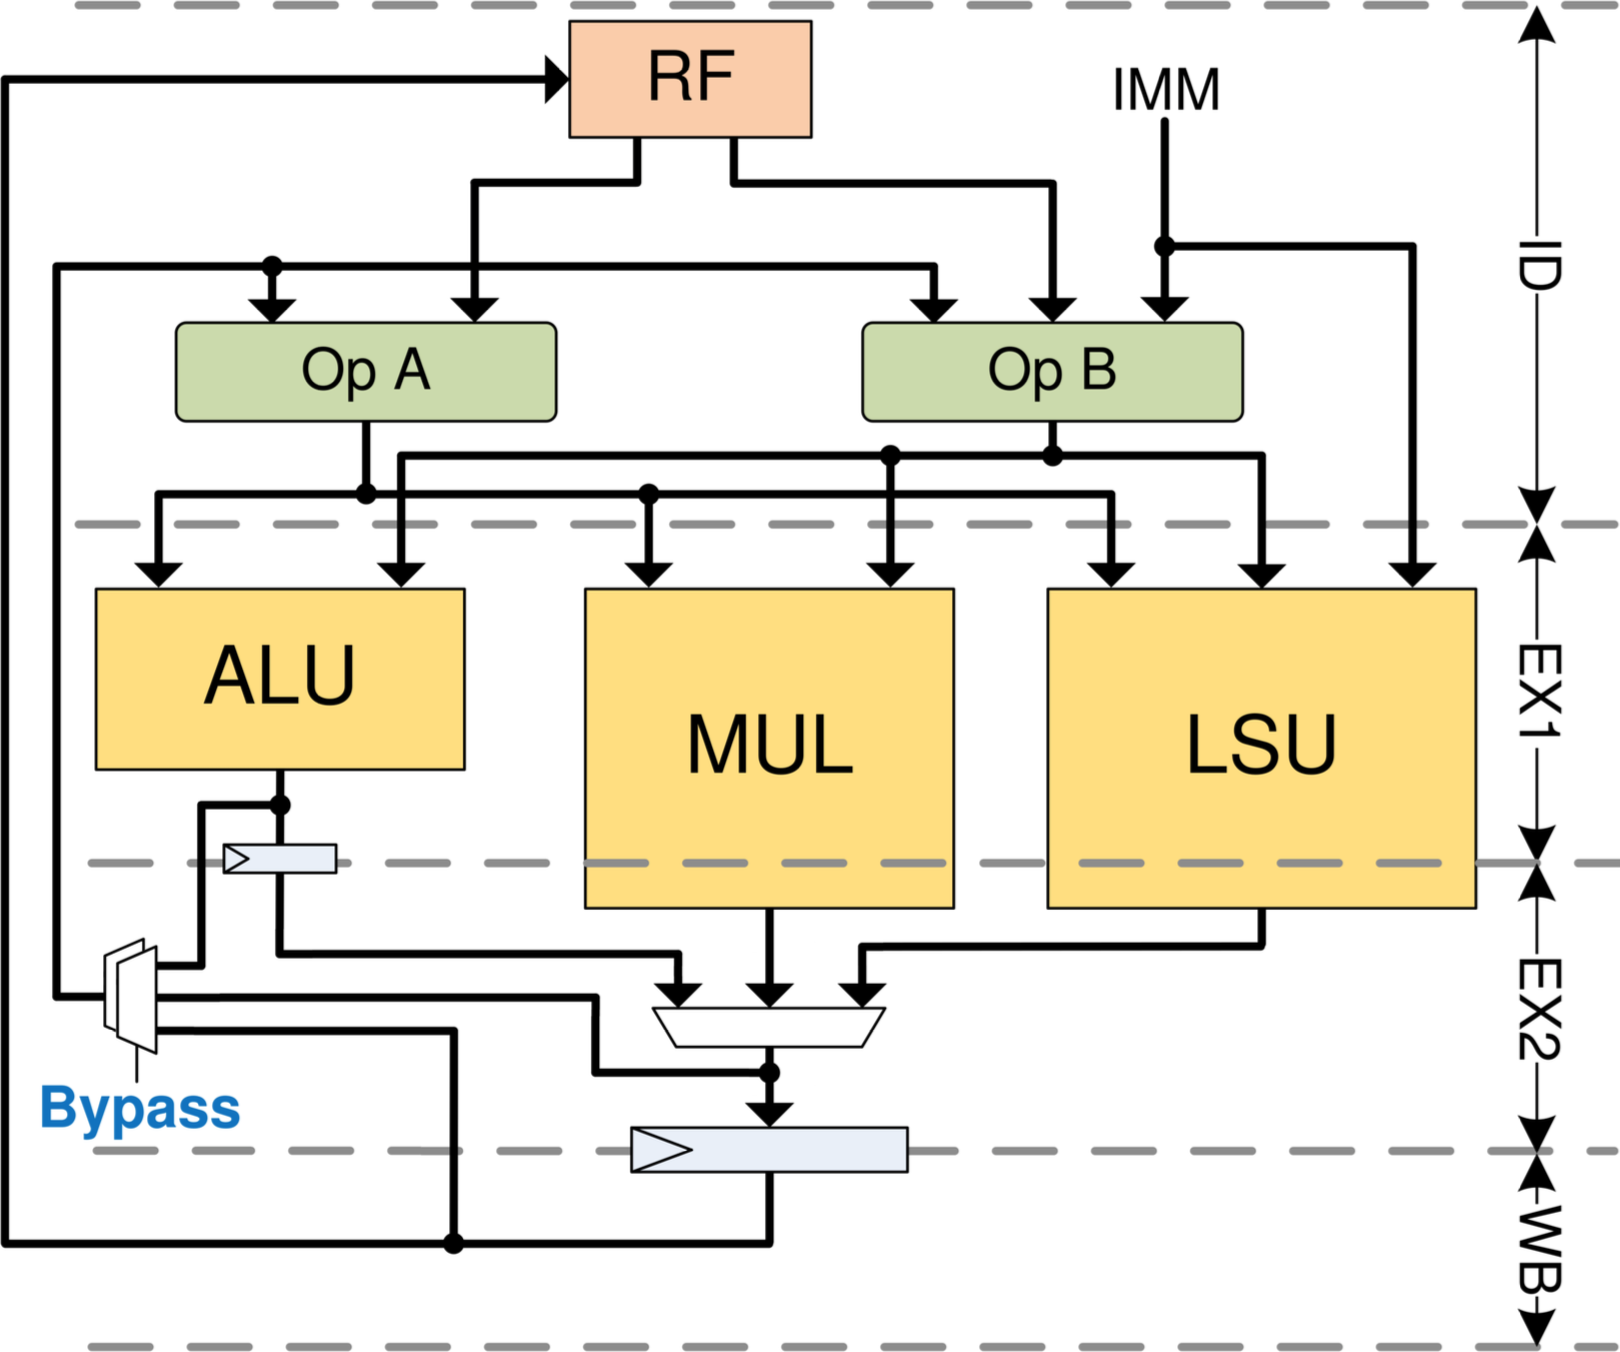
\includegraphics[width=.35\textwidth]{figures/transparent_bypass}%
\label{fig:transparent_datapath}}
\hfil
\subfloat[Datapath with explicit bypassing.]{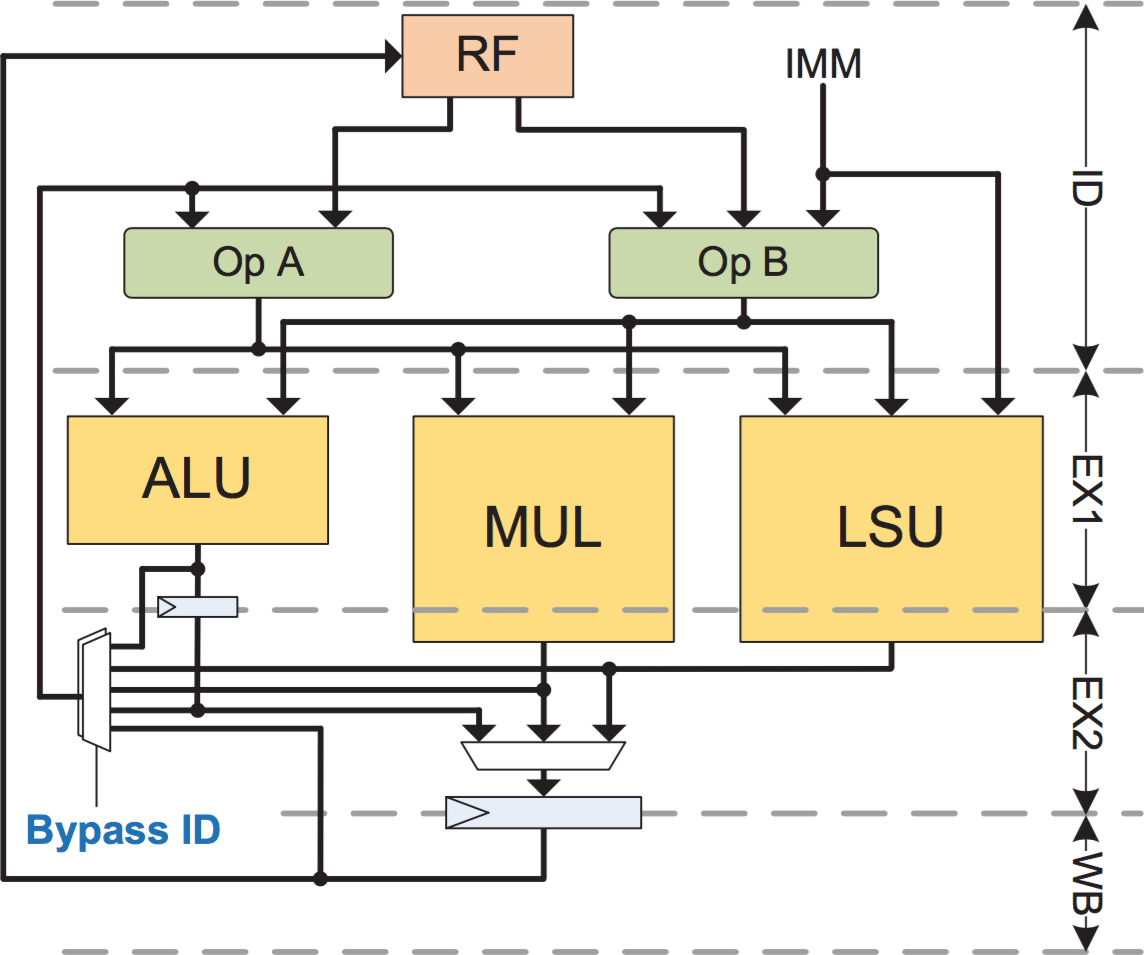
\includegraphics[width=.35\textwidth]{figures/explicit_bypass}%
\label{fig:explicit_datapath}}
\caption{Bypassing network differences between implicit bypassing and explicit bypassing.}
\label{fig:datapath_approaches}
\end{figure}

%We can configure the SIMD to have four or five stages. With four stages shown in Figure \ref{fig:4_stage}, all instructions take a single cycle, while with the five stages shown in Figure \ref{fig:5_stage}, ALU takes a single cycle, while MUL and LSU take two cycles, as shown in Table \ref{table:FU_cycles}. With 5 stages, MUL takes twice as many cycles. However, additions are simpler to perform, therefore the efficiency. 

%\begin{table}[H]
%\caption{Cycles per FU.}
%\begin{center}
%\begin{tabular}{|c|c|c|}
%\hline & \multicolumn{2}{c|}{\textbf{Cycles}} \\ \hline
%\textbf{FU} & \textbf{4-stage} & \textbf{5-stage} \\ \hline
%ALU & 1 & 1 \\ \hline
%MUL & 1 & 2 \\ \hline
%LSU & 1 & 2 \\ \hline
%\end{tabular}
%\end{center}
%\label{table:FU_cycles}
%\end{table}%

%The main difference between the two approaches is that where transparent bypassing always performs a write to a register, this is optional for explicit bypassing, as we will show in Chapter \ref{chapter:software_bypassing}.
One of the advantages of explicit bypassing is that when possible a write to a register can be avoided. Thus reducing the total energy consumption of the register file. Since there are many register files in a wide SIMD, reducing the energy consumption of the register file has a large impact on the overall energy consumption \cite{dongrio1}. Because of this, reducing the register file's energy consumption is of great importance. Furthermore, the explicit datapath shown in Figure \ref{fig:explicit_datapath} has two extra sources compared to the transparent datapath in Figure \ref{fig:transparent_datapath}. These additional bypass sources increase the chance that a result is being bypassed. In the explicit bypassing version, bypassing sources are directly accessible by the instruction. This is done by reserving part of the RF address space for the bypass sources. The disadvantage of this is that the register index space is reduced, however we do not have to change the instruction format in order to specify that an operand of an instruction is bypassed from a previous instruction.

\begin{table}[H]
\caption{Special purpose registers.}
\begin{center}
\begin{tabular}{@{}l l@{}}
\toprule
\textbf{Register} & \textbf{Purpose} \\ \hline
\emph{r0} & Constant value zero. \\
\emph{r1} & PE\_ID (PE only). \\
\emph{r3} and \emph{r4} & Return value registers. \\
\emph{r5} through \emph{r8} & Argument passing. \\
\emph{r9} & Link register (CP only). \\ 
\emph{r10} & Frame pointer. \\
\emph{r11} & Stack pointer. \\
%\multicolumn{2}{|l|}{Only with \emph{explicit bypassing}:} \\ \hline
%$R_{27}$ & $BP\_src27$ (5 stages only). \\ \hline
%$R_{28}$ & $BP\_src28$. \\ \hline
%$R_{29}$ & $BP\_src29$. \\ \hline
%$R_{30}$ & $BP\_src30$. \\ \hline
%$R_{31}$ & $BP\_src31$. \\ \hline
\bottomrule
\end{tabular}
\end{center}
\label{table:special_registers}
\end{table}%

The total number of registers grows linearly with the number of PEs because each processor has 32 registers. With a wide SIMD, we therefore have many registers that in total consume a considerable amount of energy, namely 34.6\% of the total energy consumption \cite{dongrio1}. Some of these registers have a special purpose, e.g. register $R_0$ is connected to ground is has a static value of $0$, these are shown in Table \ref{table:special_registers}.


%Todo: change this picture to have explicit and implicit bypassing instead. State then that we will be focussing on explicit bypasisng.



%Todo: add small example, having on one side normal ops. On the other hand haing implicit bypassing and finally explicit bypassing (without the store).

%\begin{figure}[b!]
%\centering
%\subfloat[4-stage pipeline with explicit datapaths.]{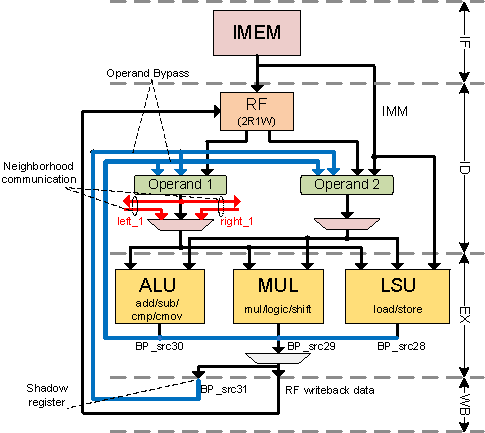
\includegraphics[width=.4\textwidth]{figures/4-stage_bypass}%
%\label{fig:4stage}}
%\hfil
%\subfloat[5-stage pipeline with explicit datapaths.]{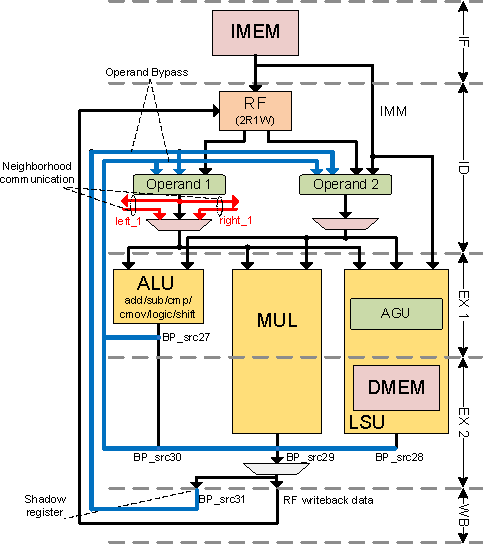
\includegraphics[width=.34\textwidth]{figures/5-stage_bypass}%
%\label{fig:5stage}}
%\caption{The pipeline of the SMD processor architecture with explicit datapaths.}
%\label{fig:pipeline_stages}
%\end{figure}

%%=============================== instruction format speech ===============================
%\section{Instruction Format}\label{sec:isa}
%%Change (optional)
%%% namely, one scalar and one vector instruction.
%%With
%%% namely, one scalar instruction that is executed on the CP, and one vector instruction that is executed on each of the PEs.
%Similar to a 2-issue VLIW instruction, an SIMD instruction consists of two subinstructions. An SIMD instruction is a 56-bit instruction that is divided up in two 28-bit subinstructions, namely, a scalar and a vector instruction. Only the CP can perform jump and branch instructions, therefore, the vector instruction can be either a R-type or an I-type instruction, while a scalar instruction can be a R-type, I-type or J-type instruction. Both sub instructions have a format, as shown in Figure \ref{fig:instruction_format}.

%\begin{figure}[H]
%\centering
%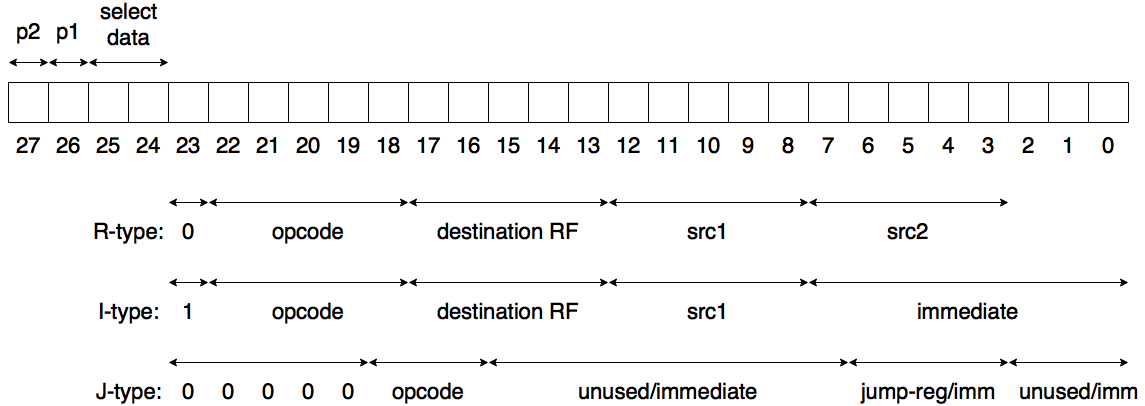
\includegraphics[width=\textwidth]{figures/instruction_format}
%\caption{Generic overview of the instruction format.}
%\label{fig:instruction_format}
%\end{figure}

%There are two guard bits $p1$ and $p2$, that can be set by using a set flag instruction. Consequently we can them for predicate execution. The instructions, branch if flag (not) set and conditional move read the predicate flag before executing. For the full overview of supported instructions, see Appendix \ref{chapter:supported_operations}.

%Note that the "select data" bits are also part of the instruction as we explained in Chapter \ref{sec:nn}. The CP and PEs can communicate by setting these bits. The communication model is shown in Table \ref{table:select_data}.


%\clearemptydoublepage

%\chapter{The LLVM Infrastructure}\label{chapter:llvm}
%The LLVM project started in 2000 by Chris Lattner, as a research project at the University of Illinois with the goal of providing a modern, Static Single Assignment (SSA)-based compilation strategy capable of supporting both static and dynamic compilation of arbitrary programming languages. It was first released in 2003, although the project has grown rapidly since then. It has become popular amongst major companies, e.g. Google, Apple and Sony, for its powerful multi-stage compilation strategy and outstanding extendibility. LLVM is a collection of modular and reusable compiler and toolchain technologies. Generally, LLVM follows a 3-phase design, which is divided up in a frontend, a code independent optimizer and a backend, illustrated in Figure \ref{fig:3phase_design}.

\begin{figure}[H]
\centering

\includegraphics[width=.7\textwidth]{figures/3phase_design}
\caption{3-phase design: frontend, optimizer and backend.}
\label{fig:3phase_design}
\end{figure}

%Reorder list: [IR, Lexical analysis, Syntax analysis, ]
\textbf{The frontend} is responsible for translating code of an arbitrary language into LLVM's Intermediate Representation (IR) code. The LLVM instruction set represents a virtual architecture that captures the key operations of ordinary processors, but avoids machine specific constraints such as physical registers. Instead, it has an infinite amount of virtual registers in SSA form, which means that each virtual register is assigned only once and each use of a variable is dominated by that variable's definition. This simplifies the dataflow optimizations because only a single definition can reach a particular use of a value, and finding that definition is trivial \cite{llvm_strategy}.
%frontend talk, straight from the Dragon Book plz.
%introduce parser and lexical analysis and that it is kept in an AST, which will be translated as a final step to IR.
%Perhaps an example?
%TODO: rewrite first sentence in my own words.
As the first phase of a compiler, the main task of the lexical analyzer is to read the input characters of the source program, group them into luxemes, and produce as output a sequence of tokens. These tokens are used by the parser for syntax analysis, where we verify that the sequence of tokens can be reconstructed according to the syntax of the input language. The parser should report any syntax errors during this process and should be able to recover in order to continue processing the rest of the program. The parser constructs a parse tree, and the semantic analyzer uses this parse tree to check for consistency with the language definition. Type checking is also done during this stage, and the information is kept in the syntax tree. The result of these phases is an Abstract Synctax Tree (AST) of the program, which can be translated into three-address IR code. %We will discuss LLVM's IR in more detail in Chapter \ref{sec:ir}

\textbf{The optimizer} contains a collections of analysis and semantic-preserving transformations that can be used to optimize IR code. One of the advantages of LLVM is that when you build a new backend for any given processor architecture you immediately have access to all of these optimizations. Below we give some of these optimizations that are explained more detailed in literature \cite[Chapter~9]{dragon_book}.%TODO: provide chapter in cite.
\begin{itemize}
\item \emph{Constant propagation} computes for each point and each variable in the program, whether that variable has a unique constant value at that point. This can then be used to replace variable references with constant values.
\item \emph{Constant folding} recognizes and evaluates constant expressions at compile time rather than runtime. For example, `$add\ 1+2$' can be replaced by `$3$'. Statements like `$add\ 1+2$' can be introduced by other optimizations, e.g. constant propagation. 
\item \emph{Common sub-expression elimination} recognizes that the same expressions appears in more than one place, and that performance can be improved by transforming the code such that the expression appears in one only place.
\item \emph{Copy propagation} replaces each target of a copy statement with that of the copied value. For example, if we have a copy statement, $x = y$. Then the uses of $x$ can be replaced by $y$. Some optimizations require that this optimizations is performed afterwards to cleanup, e.g. common sub-expression elimination requires this pass to run afterwards. 
\item \emph{Dead code elimination} removes code that do not affect the programs results. This avoids executing irrelevant operations and reduces the code size of a program.  
\item \emph{Loop invariant code motion} aims at moving code that is independent of the loop iteration out of the loop body. It does this by moving the loop independent statement above the loop, saving it in a temporary variable, and use it in each iteration of the loop. Now the loop independent statement is computed only once instead of every iteration. 
\item \emph{Function inlining} verifies whether inlining functions in its callees gives a performance benefit. If doing this would give performance benefit, it replaces the call of the function with the function body. This optimization often is useful for small functions because it reduces the overhead that is introduced when a function call is made, e.g. storing frame pointer, storing function parameters and jump in code to where the function is defined.     
\end{itemize}

\begin{figure}[b!]
\centering
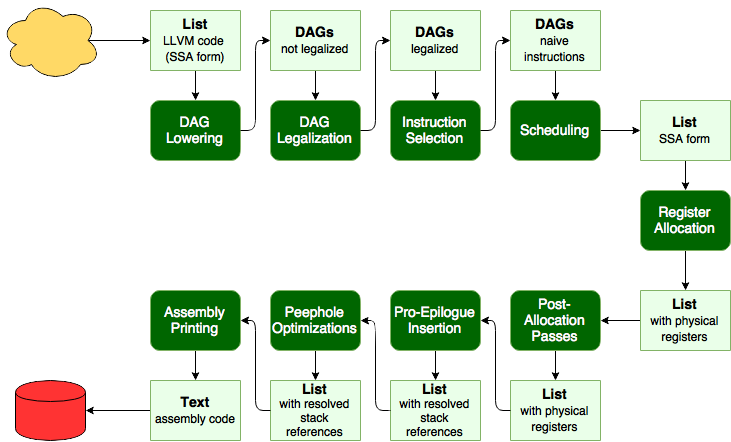
\includegraphics[width=\textwidth]{figures/code_generation_sequence}
\caption{Code generation sequence, from LLVM code to assembly code.}
\label{fig:code_generation}
\end{figure}

%TODO: apply following namings: Instruction, Machine instruction, scheduled instruction in SSA form, schedule instruction not in SSA form.
\textbf{The backend} translates, according to a processor architecture, IR code to a target specific assembly language. It does this by going through a sequence of code generation stages, illustrated in Figure \ref{fig:code_generation}. The rectangular boxes indicate the data structure that is used by, and produced by a given stage, and the name of each stage is denoted in a rectangular box with rounded corners. During this process, first the IR code is lowered to a Directed Acyclic Graph (DAG) in which each node represents one instruction. However, for some architectures, not all data types and instructions are supported. For this reason, the DAG is legalized to something that is supported by the target architecture. Instruction selection maps each of the nodes into machine nodes, by matching patterns. %After that, the instruction selector maps the pattern of LLVM code into the target machine code and builds a new DAG whose nodes represents the target instructions.
Then we have a DAG consisting of only target specific machine instructions, in SSA form. Having naive machine instruction, the next step is to schedule them. We schedule the machine instructions according to the resource information of the target processor, and assign each instruction to a specific cycle. 
%We will discuss scheduling in more detail in Chapter \ref{sec:scheduling}. 
Now the instructions are represented in a list rather than a DAG, but still in SSA form. The Register Allocator (RA) then assigns physical registers to each of the virtual registers, now the list is not in SSA form. 
%We will discuss RA in more detail in Chapter \ref{sec:register_allocation}. 
The post-allocation pass can improve the schedule, taking the physical registers and register pressure, that is known at this point, into account. After that, some epilogue and prologue code might need to be inserted, e.g. saving/restoring the caller/callee registers and reserving/destroying of the function's stack frame. The peephole optimizations are target specific improvements to the schedule that has been constructed. These optimizations deal with very specific optimizations that can only be done at the end of the process. At last, the assembly printer, prints the assembly code.
%backend talk -> huuge



%\subsection{Instruction Scheduling}\label{sec:scheduling}
%After instruction selection, the program is represented in SSA form as a DAG. Each instruction is represented as a $MachineSDNode$ in a $MachineBasicBlock$. After scheduling has been performed, each instructions now is represented as a $MachineInstr$. 



%ach instruction is scheduleDuring instruction schdduling, each $MachineBasicBlock$ is scheduled by the scheduler and transformed into a $MachineInstr$. After this phase, instructions are represented as $MachineInstr$.

%\subsection{Register Allocation}\label{sec:register_allocation}
%Register allocation is executed during the code generation phase and consists of finding a mapping of a program with an unlimited number of virtual registers to a program with a limited number of physical registers.
%Examples, machine instrs on the left in SSA form, on the right with proper registers next to it.
%Introduce at least 

\subsection{Scheduling and RA}
TODO: exlain phase ordering between scheduling and RA, from ref \cite[Chapter~10.2.4]{dragon_book}.

Introduce terms spilling, register pressure, and use this reference \cite{ra}.




%Additional ref. 
%






%\clearemptydoublepage

\chapter{Related Work}\label{chapter:related_work}
There is related work for compilers that target SIMD architectures, in particular, a compiler has been developed, referred to as legacy compiler. Furthermore, there is related work in building an LLVM backend, and compiling with explicit data paths has been an active research topic for other architectures. We will also discuss some related work in scheduling and register allocation. We have divided this in four section in the remainder of this chapter.
% scrap
%The related work is introduced in this part, including the legacy compiler, building the LLVM back-end for SIMD architecture, explicit datapaths in other architecture and some scheduling and register allocation algorithms applied in other compilers.

\section{Legacy compiler}
The legacy compiler was developed by the ES group in 2003. We will use the SIMD architecture as it was designed during that project \cite{simd}. The legacy compiler has a custom backend for the SIMD architecture, that can generate code for explicit data paths \cite{dongrio1} and it can only compile a subset of C code and hand-touched OpenCL code, which requires manual insertion of custom pragmas to compile efficiently \cite{dongrio2}, which we do not desire. Our goal is to overcome these limitations and improve the compilers maintainability. Furthermore, the new compiler will be evaluated relative to the legacy compiler in order to access efficiency of the generated code.
%Dongrio's simd work 
%Johan janssen & ... TTA work
%Other exposed datapaths

\section{Building an LLVM back-end}
Our backend is derived from tricore tutorial on creating a new backend for the LLVM compiler framework \cite{tricore}. Furthermore, based on that work, an LLVM backend for SIMD architecture without explicit bypassing has been developed \cite{liu_zhenyuan}. However, the current compiler generates code with implicit bypassing. We, therefore, need to extend this to efficiently generate code for explicit bypassing as well. Therefore, our work will be an extension to previously noted work.

\section{Other Exposed/Explicit Datapath Architectures}
Compiling with explicit data,paths have been an active topic of research. We have investigated several architectures that face similar challenges. One of the main works that we investigated is the TTA architecture, where instructions consist of data transports. However, their approach can not be used because with our SIMD architecture, data transports are given and we want to compile in order to efficiently use the explicit data paths that are provided \cite{tta, tta_codegen}.

Another architecture that exploits explicit datapath architectures is the ReMove architecture \cite{remove}. That work focusses on scheduling for partially connected architectures with explicit data paths. The ReMove architecture is similar to a VLIW, having multiple FUs, however here they have an interconnect network that connects the FUs to the RF. The scheduling algorithm used in this work can not be used in our work, because similar to the legacy compiler for SIMD, this project has a custom backend, which can not be reused for LLVM. However, the basic principles of the scheduling algorithms proposed in this work are still valid and may be reused for our work.

\section{Scheduling and Register Allocation}
First of all, from the existing scheduling algorithms, Swing Modulo Scheduling (SMS) seems to be a suitable scheduling approach. It is a heuristic approach that is able to deal efficiently with software pipelining. Furthermore, it is known for its outstanding performance and low computational cost. The generated schedules are near optimal in terms of initiation interval and register requirements \cite{swingmodulo_paper, swingmodulo_thesis}. We consider this a candidate scheduler to use.

Furthermore, the following literature discusses register allocation for SSA-based programs that solves coloring problem optimally in quadratic-time optimal by decoupling coloring, spilling and coalescing \cite{ra}. This technique may allow us to implement a custom register allocator that solves the problem in polynomial time.

Finally, there is another project, called Unison. They solve scheduling and register allocation and other code generation tasks by translating them into combinatorial problems and solve them together with constraint programming \cite{unison}. We consider this a candidate constraint solver to use because it can be easily integrated with LLVM.

%\clearemptydoublepage

\chapter{Explicit Bypassing}\label{chapter:explicit_bypassing}
Suppose that we have a four stage pipeline where each instruction takes only one cycle. Let $a$ and $b$ be two instructions with a R/W dependency, i.e. instruction $b$ uses a value that is defined by instruction $a$. During the first cycle, instruction $a$ is fetched from Instruction Memory (IMEM). In the second cycle, instruction $a$ selects the operands from the RF, and instruction $b$ is fetched from IMEM. During the third cycle, instruction $a$ is in the execution stage, while instruction $b$ selects the operands that it needs. During the fourth cycle, instruction $a$ is in the WB stage, where it writes the result back to the RF, and instruction $b$ is in the execution stage.

Without bypassing, the result of instruction $a$ will be available only after it is written back. On the other hand, when we do have a bypass network, we may forward the result of an instruction to another instruction. In our example, we have forwarded the result of instruction $a$ directly to the operand of instruction $b$, as indicated by the vertical arrow that goes from the first to the second instruction in Figure \ref{fig:bypass_principle}. A result of an instruction may be accessed a cycle earlier when we compare with and without bypassing, however the target architecture has either explicit or implicit bypassing, which are both access a result a cycle early. So, in terms of cycles it makes no differences whether to use explicit or implicit bypassing. However, as you will see later, explicit bypassing has an advantage over implicit bypassing.

\begin{figure}[H]
\centering
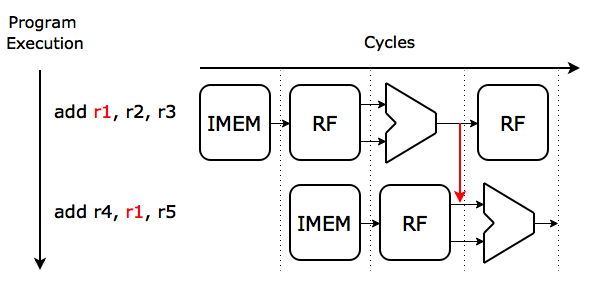
\includegraphics[width=.6\textwidth]{figures/bypassing_principle/05_bypassing_principle}
\caption{Illustration of bypassing and software pipelines in general.}
\label{fig:bypass_principle}
\end{figure}

With bypassing, we have wires that connect outputs of EX stage to the ID stage and we have this for each bypass source. 

\section{Implicit Bypassing}
With implicit bypassing we have wires that connect the outputs from EX stage to the ID stage, as illustrated in Figure \ref{fig:impl_bypass_principle}. Furthermore, we also have wires that go from the WB stage to the ID stage, however this is not shown in this example. To detect bypasses, the HW matches whether the operands of the currently issued instruction to the destination address of previously issued instructions. If we have a match, and the result is still available in the pipeline, we can then bypass it. We have a mux that controls which inputs are used, i.e. a value from a register, or a value from a bypass. The bypass detection hardware is in control which of these values is selected.

\begin{figure}[t]
\centering
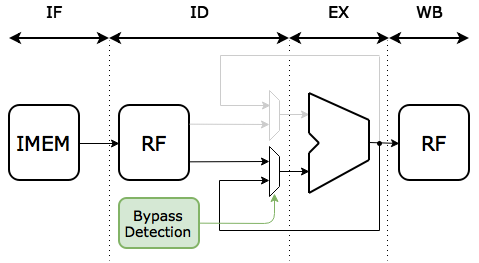
\includegraphics[width=.5\textwidth]{figures/impl_bypassing_principle/03_implicit_bypassing_principle}
\caption{Illustration that shows the basic principles of implicit bypassing.}
\label{fig:impl_bypass_principle}
\end{figure}

\section{Explicit Bypassing}
For explicit bypassing, we have similar wires that connect outputs of EX stage to the ID stage as we have in implicit bypassing. However, with explicit bypassing the compiler is responsible for detecting when we can bypass the result of a instruction. In Figure \ref{fig:exp_bypass_principle_r} we show that the control signal to the mux, that selects the input from a register or from a bypass, is now controlled by the compiler. The compiler encodes this information in an instruction. This way, during instruction decoding, the control signal is immediately available. Furthermore, we have a read-enable flag on the register file. If we then want to take the data from a bypass, we can set this value to zero. This way, we can avoid speculative reads accesses from the RF. We use the same signal from the ID stage, to control the read-enable on the register file and the signal that controls the mux. 

\begin{figure}[H]
\centering
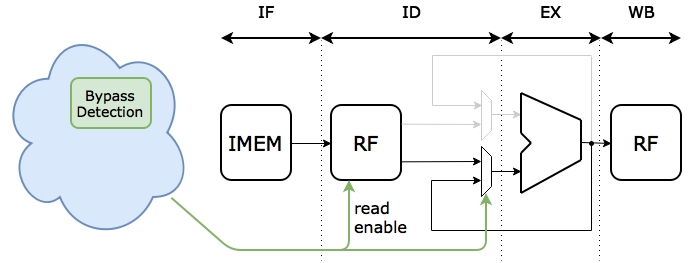
\includegraphics[width=.7\textwidth]{figures/expl_bypassing_principle/01_explicit_bypassing_principle}
\caption{Illustration that shows the basic principles of explicit bypassing, read enabled port on RFs to avoid unnecessary reads.}
\label{fig:exp_bypass_principle_r}
\end{figure}

We can use the liveliness information during compilation to determine whether a variable is live after it is used. If the variable is not live after it is used often indicated by a kill of a variable, we can disable the write on the register, since it will not be needed anymore. Figure \ref{fig:exp_bypass_principle_rw} illustrates this by adding a write-enable flag on top of the read-enable that was already present from Figure \ref{fig:exp_bypass_principle_r}. Adding a write-enable flag allows us to avoid speculative write accesses to the RF.

\begin{figure}[t]
\centering
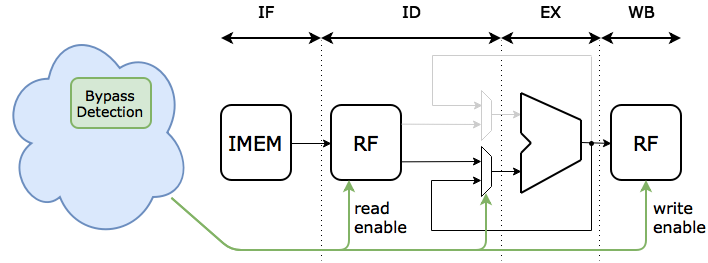
\includegraphics[width=.7\textwidth]{figures/expl_bypassing_principle/02_explicit_bypassing_principle}
\caption{Illustration that shows the basic principles of explicit bypassing, read enabled port on RFs to avoid unnecessary reads and write enable port to avoid speculative writes.}
\label{fig:exp_bypass_principle_rw}
\end{figure}

A significant difference between explicit and implicit bypassing is that some writes accesses to the register file may be avoided for explicit bypassing, while this is can not be done with implicit bypassing.

In general, the result of an instruction will remain in the pipeline  scheduled in the future, in order to see whether the result of an operation will be used later on, which is not possible at runtime.

%%%%%%%%%%
%\section{Bypass Sources}

The target architecture has operand isolation, which we mentioned in Chapter \ref{sec:processor}. Because of this, the output of the function units do not toggle, i.e. are only calculated when the operand registers change. This has as a side effect that when a function unit is not used, the output register remains the same. This means that a instruction can be bypassed, as long as we do not use the function unit on which it was executed. We have given the bypass sources for our architecture below, in Table \ref{table:bypass_alias}. Here we have provided all bypass sources for the four stage and five stage pipeline

\begin{table}[H]
\caption{Alias for each bypassing source, $BP\_src$ in Figure \ref{fig:4_stage} and Figure \ref{fig:5_stage}.}
\begin{center}
\begin{tabular}{@{}llll@{}}
\toprule
\multirow{2}{*}{\textbf{Register:}} & \multirow{2}{*}{\textbf{Bypass source:}} & \multicolumn{2}{c}{\textbf{Alias}:} \\ \cline{3-4}
 & & \textbf{4 stages} & \textbf{5 stages} \\
\hline
\emph{r27} & $BP\_src27$ & N/A & ALU1 \\ 
\emph{r28} & $BP\_src28$ & LSU & LSU \\
\emph{r29} & $BP\_src29$ & MUL & MUL \\ 
\emph{r30} & $BP\_src30$ & ALU & ALU2 \\
\emph{r31} & $BP\_src31$ & WB & WB \\
\bottomrule
\end{tabular}
\end{center}
\label{table:bypass_alias}
\end{table}%

%%%%%%%%%%%%

We will now show with an example that avoiding speculative write accesses may reduce Register Pressure (RP).

%TODO: move this to a better place, or explain this in one of the previous sections
%this being that we have multiple bypassing sources, we specify them as if they were a register, and the following registers map to the following bypassing sources.
%One from each FU, one from WB and an additional one from blala
%With automatic bypass we actually always bypass from WB, because otherwise each instruction would take one more cycle. Namely one or two execution stages and a wb stage after which the result is the register.
%With explicit bypassing the compiler can avoid some accesses to RFs by explicitly specifying the datapath.

%Connect to TTA architectures, use findings of Johan Janssen.

%Show the need for this like done in Johans' paper. (and in lucs paper)

%Different approches
% - Naive implementation
% - Scheduling pass to automate it
% - Combine RA and scheduling to do it better.
% - Use LLVMs way to describe explicit bypassing, namely targetItinirary.td

\begin{lstlisting}[caption=Example code fragment where no bypassing is specified., label=lst:nobypass]
mul <@\textcolor{red}{r1}@>, r2, r3
add r4, <@\textcolor{red}{r1}@>, r5
\end{lstlisting}

Listing \ref{lst:nobypass} shows a code fragment with a multiplication and an addition. We have a flow dependent dependency. Namely, the result of the multiplication is used by the addition.

\begin{lstlisting}[caption=Example code fragment avoiding a read access., label=lst:operandbypass]
mul <@\textcolor{red}{r1}@>, r2, r3
add r4, <@\textcolor{red}{MUL}@>, r5
\end{lstlisting}

In Listing \ref{lst:operandbypass} we have replaced the use of $r1$ with $MUL$. This indicates that we do not take the first operand from the RF, but from a bypass instead. Since we obtain the result of the multiplication from the bypass network, we do not require a read access to $r1$ anymore.
%This is also done for the implicit bypassing approach, however since we have more bypass sources for the explicit bypassing variant, we expect that operand bypassing is done more aggressively.

\begin{lstlisting}[caption=Example code fragment avoiding a read and a write access., label=lst:fullbypass]
mul <@\textcolor{red}{--}@>, r2, r3
add r4, <@\textcolor{red}{MUL}@>, r5
\end{lstlisting}

When the result of $r1$ is not needed anymore, for example, the live range of $r1$ spans no further than this addition, the write access can be avoided. By specifying $--$ as destination, the result will not be written back, as illustrated in Listing \ref{lst:fullbypass}. Register $r1$ is now completely removed from the example, effectively freeing that register. We have now reduced RP by one, since we require one less register. The freed register can be used for other calculations, which may lead to a higher performance.

%%%%%%%%%%%%%%%%%%%%%%%%%%%%


%HERE WE SHOW ALL DIFFICULT CASES, i.e. First instruction of loop body is bypassed from last instruction of loop body.
\section{Joint Point Issue}
In the following example we will illustrate a special case that may be taken into consideration.

\begin{lstlisting}[caption=Example code fragment where bypassing over backedge of a loop iteration is not possible., label=lst:bypassloop1]
      lw <@\textcolor{red}{r6}@>, r10, 5
loop: 
        <@\raisebox{-1pt}[0pt][0pt]{$\vdots$}@>
      
      sfeq <@\textcolor{red}{r6}@>, r0
      bnf loop
      addi <@\textcolor{red}{r6}@>, <@\textcolor{red}{r6}@>, -1

        <@\raisebox{-1pt}[0pt][0pt]{$\vdots$}@>
\end{lstlisting}

When we access the loop counter for the first time in Listing \ref{lst:bypassloop1}, $r6$ can be bypassed from the $LSU$. However, in consecutive iterations, we would bypass it from the $ALU$ instead. Listing \ref{lst:bypassloop2} shows that adding an instruction before entering the loop allows us to bypass the value in consideration. We may profit from this if a lot of loop iterations are processed.

\begin{lstlisting}[caption=Example code fragment where bypassing over the backedge of a loop iteration is possible., label=lst:bypassloop2]
      lw <@\textcolor{red}{--}@>, r10, 5
      add <@\textcolor{red}{r6}@>, <@\textcolor{red}{LSU}@>, 0
loop: 
        <@\raisebox{-1pt}[0pt][0pt]{$\vdots$}@>
      
      sfeq <@\textcolor{red}{ALU}@>, r0
      bnf loop
      addi <@\textcolor{red}{--}@>, <@\textcolor{red}{r6}@>, -1

        <@\raisebox{-1pt}[0pt][0pt]{$\vdots$}@>
\end{lstlisting}

%TODO: leg dit eens fatsoenlijk uit joh
Here we want to apply bypassing to bypass the result of the last add instruction in the loop before we branch to the first instruction in the loop. However, when we go in the loop for the first time, $r6$ comes from the LSU instead of the ALU. Therefore, sometimes it is necessary to insert an instruction before we enter a loop to bypass over loop iterations.

%\section{Proposed Approaches}
%We will investigate in different approaches to implement software bypassing on top of the SIMD architecture within LLVM. Each of these approaches will be evaluated. The kernels that we will use as means of evaluation are discussed in Chapter \ref{sec:benchmark}.

%\begin{enumerate}
%\item Naive approach in which we will add a pass on top of the existing scheduler to apply software bypassing whenever possible. In this approach, explicit datapaths are created after scheduling and register allocation.
%\item Use LLVMs framework to express the processors pipeline stages and bypassing sources. This way LLVM will apply software bypassing. This will be a good reference for our final approach.
%\item Implement a bypass aware combined scheduling and register allocation algorithm. We need to investigate what steps need to be taken to implement a custom scheduler in LLVM.
%TODO: introduce the need for combined scheduling and RA..... 
%\end{enumerate}
%Incorporate notes from 21/22 februar, write a long text to discuss all of them. This way we have motivation for each of the proposed solutions.

%TODO: make example for each approach.

%\section{Method of Evaluation}\label{sec:benchmark}
%Discuss the kernels that we will use to evaluate the different approaches. We will use RTL synthesis to emulate the processors behaviour on certain kernels and model the energy consumption for each of the approaches, for the transparent bypassing variant, and finally for a by hand optimized and bypassed variant. This should give us an "optimal" energy reduction compared to the energy reduction that we achieved, with transparent bypassing as reference.




%\clearemptydoublepage

\chapter{Proposed Solutions}\label{chapter:solutions}
Our approach to implement explicit bypassing to fit it in our compiler within LLVM is to allocate the available bypasses sources during one of the compiler stages. The major compilation phases in LLVM are illustrated in Figure \ref{fig:phase_ordering}.  The first block represents instruction legalization, instruction lowering and instruction selection, In general, we have that first the instructions are scheduled, then register allocation (RA) is performed, and finally the instructions are printed in assembly language. Although one can use a post-RA scheduler to change the order in which to do scheduling and register allocation. At some point, we have to allocate our bypasses, which we can do only after we have backend specific instruction, i.e. after instruction selection. However, we could do this during any of compilation stages that follow, i.e. before scheduling and register allocation, during scheduling and register allocation and at the end of compilation. Moreover, scheduling and register allocation is already a phase problem on its own, as we have mentioned in Chapter \ref{sec:scheduling_and_ra}. Altogether, this leads to many possible approaches and we will discuss some of them below.

\begin{figure}[H]
\centering
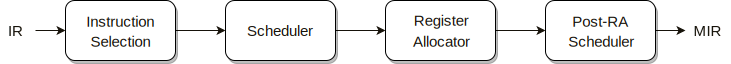
\includegraphics[width=.15\textwidth]{figures/phase_ordering}
\caption{Generalized code generation sequence.}
\label{fig:phase_ordering}
\end{figure}

\section{Last-minute Allocation}\label{sec:last_minute_alloc}
%Approach 1
One approach would be to allocate bypasses during the last stage of the compiler, just before printing the instructions. At this point, instructions are in order of execution and register allocation has already been performed and spill code has already been inserted in case we ran out of registers during RA. Because the order of instructions does not change at this point, the advantage of this approach is its simplicity. Namely, we could implement a pass that works on basic blocks, a basic block is a sequence of instructions with no branches, except for entering and leaving the basic block.

We could implement a pass to our backend that keeps track of the state of our pipeline in order to allocate our bypasses. Then we can determine for a cycle, which values currently reside in our bypass registers. Using this information we can then allocate bypasses andprocess the instructions in a top-down approach, demoting physical registers into bypass registers.

However, when we ran out of registers during register allocation, we had inserted spill code. When we allocate bypasses, we effectively free up registers. Since the spill code had already been inserted, it might have become unnecessary. Therefore, one improvement to this approach would be to move spill code after bypasses have been allocated to where they are needed, in order to avoid unnecessary spills.

\section{Bypass-aware Register Allocation}\label{sec:ra_approach}
%Approach 2
Another approach would be to implement a bypass-aware register allocator. Assuming that we have performed scheduling before register allocation, the instructions are in order of execution, allowing us to model the pipeline state as we did for the first approach. Our bypass-aware register allocator could start by allocating bypass registers. Then the remaining virtual registers could be allocated as usual. With this approach, we reduce register pressure by allocating bypasses before register allocation, effectively freeing registers. Therefore we may need less spill code, which is now inserted after bypasses have been allocated. So in contrary to the first approach, we do not have to take special care of spilling.

This approach would require us to implement a custom register allocator that consists of two phases. First, we allocate a bypass registers for each virtual register that can be bypassed. Subsequently, we have to allocate physical registers for the remaining virtual register. For the second phase we may reuse any of the existing register allocators. 
%Introduce example code where we could have better bypass utilizzation, i.e. less stores by scheduling differently

\section{Bypass-aware Scheduling}\label{sec:scheduling_approach}
%Approach 3
For this approach we need to implement a custom scheduler for our backend. This scheduler would prioritize to schedule instructions that may be bypassed close to each other, such that we may increase the possible number of bypasses. If we were to allocate bypasses during scheduling, code might be inserted during register allocation or any other passes that follow, that may break a previously allocated bypass. Therefore, it may be wise to allocate the bypasses as late as possible, and let the scheduler be responsible for improving utilization of the bypass network. 


\section{Pre Scheduling Allocation}\label{sec:pre_scheduling}
%Approach 4
Before scheduling, we can identify instruction pairs that we can bypass. Then we change the virtual register that is bypassed into bypass registers and glue the two instructions together. This however makes restrictions on the resulting schedule. Since we group instruction together before scheduling, we may improve utilization of the bypass network. Namely, we may have grouped instruction together that otherwise would be scheduled far apart. This approach requires some new heuristics to determine whether it is profitable to group instruction together or when this may decrease efficiency, i.e. when grouping instructions decreases available ILP. 

When we allocate bypasses before scheduling and register allocation, it is possible that the scheduler or register allocator reorder instruction, or insert instruction, e.g. spill code, which breaks a previously allocated bypass. Therefore, a better approach would be to group instructions together as explained above, but allocate the bypasses as late as possible, similar to the previous approach.

With this approach, we would need to find a tradeoff to not restrict the schedule too much, but still utilizing the bypass network as much as possible.   

\section{Combined Scheduling and Register Allocation}\label{sec:combined_sched_ra}
%Approach 5 & 6
We can also choose to solve scheduling and RA in one go. This way, problems that can arise of doing one before the other may be avoided. There are two approaches to solve this problem. One is to solve it optimally, using constraint programming. Unison, a separate project that solves scheduling and register allocation optimally in one go can be used with LLVM and can be extended to allocate our bypasses. However, solving this problem optimally, may increase compilation time significantly, which we would like to avoid. Therefore, another approach would be to use heuristics to solve scheduling and register allocation in one go. There are no implementations of this thus far, which makes this approach the most difficult one. However, when we can efficiently deal with these problems in one go, we might extend this for other architectures as well. 

%\clearemptydoublepage

\chapter{Planning}\label{chapter:planning}
Coarse-grain and fine-grain planning for the graduation phase. The graduation phase will take six months, so we distribute that time span over each of the phases in Table \ref{table:planning}.

\begin{table}[h]
\caption{Time table for the graduation phase.}
\begin{center}
\begin{tabular}{@{}p{0.25\textwidth-2\tabcolsep}p{0.6\textwidth-2\tabcolsep}p{0.15\textwidth-2\tabcolsep}@{}}
\toprule
\textbf{Phase} 		& \textbf{Tasks} & \textbf{Duration} \\ \hline
Benchmarks setup 	& Develop benchmarks described in Chapter \ref{chapter:evaluation}.			& 1 week \\
First phase		& Implement a pass that allocates bypasses last minute, just before instructions are printed, as described in Chapter \ref{sec:last_minute_alloc}.		& 1 week \\
Second phase	& Implement a custom register allocation, that first allocates bypasses and allocates the remaining registers as usual, as described in Chapter \ref{sec:ra_approach}.	& 2 weeks \\
Third phase		& Implement a custom scheduler for our backend, that improves utilization of the bypass network, as described in Chapter \ref{sec:scheduling_approach}. & 3 weeks \\
Fourth phase 	& Implement a pass glueing instructions together that can be bypassed, as described in Chapter \ref{sec:pre_scheduling}. & 3 weeks\\
Fifth phase 	& Extend Unison to make it bypass aware, as described in Chapter \ref{sec:combined_sched_ra}. & 3 weeks \\
Sixth phase		& Implement heuristics that do combined RA and scheduling, as described in Chapter \ref{sec:combined_sched_ra}. & 5 weeks \\
Final report		& Write report and collect benchmark data. 	& 6 weeks \\
\hline%\cline{3-3}
\multicolumn{2}{c}{ \multirow{2}{*}{Total time}} 				& 24 weeks\\
	&											& (6 months)\\
\bottomrule
\end{tabular}
\end{center}
\label{table:planning}
\end{table}%


%\clearemptydoublepage

\chapter{Conclusions}\label{chapter:conclusions}
The implementation of a SIMD compiler based on LLVM infrastructure has been described in the previous chapters. This chapters summarizes the results, shows the limitations of the compiler, and presents future work.

\section{Summary}
\Blindtext

\section{Future Work}\label{sec:future_work}
Optimalisaties en ander werk (e.g. disassembler) dat ik tegen kom, maar geen tijd voor heb om te implementeren/buiten de scope v/h project valt komt hier.

Als dit een klein hoofdstuk wordt (<2 paginas) dan kan deze worden samegevoegd met de Conclusie in Hoofdstuk \ref{chapter:conclusions}. 

\blindtext

\Blindtext



%In general a short summarizing paragraph will do, and under no circumstances should the paragraph simply repeat material from the Abstract or Introduction. In some cases it's possible to now make the original claims more concrete, e.g., by referring to quantitative performance results.

%Old text
%We have implemented last-minute bypass allocation and tested it on some benchmarks. However, we do not yet have all the benchmarks that we intend to use. Therefore we do not yet have reliable results that could indicate how efficient our first approach is. Furthermore, we have implemented last-minute bypassing for code generation, where we use only the CP processor. We want to extend this to allocate bypasses in a basic block for code generation, where we use both CP and PEs.

%The overall results are good, however, there are some limitations. Our approach processes basic blocks with only the available information of the current basic block. We notice that bypassing opportunities may be missed for small basic blocks, having only a few instructions. %This could be resolved however, by splitting the current pass in an analysis pass and a transformation pass. We then run the analysis part first, so that we have the state of 


%BEGIN PROS & CONS
%We have evaluated each of the proposed solutions on their tradeoffs in table \ref{table:tradeoffs} on estimated implementation effort, compilation times if the approach were used, and gain in code quality that we may expect for each of the solutions. 

%\begin{table}[h]
%\caption{Table with tradeoffs for each approach from Chapter \ref{chapter:solutions}.}
%\begin{center}
%\begin{tabular}{@{}p{0.4\textwidth-2\tabcolsep}p{0.2\textwidth-2\tabcolsep}p{0.2\textwidth-2\tabcolsep}p{0.2\textwidth-2\tabcolsep}@{}}
%\toprule
%\textbf{Aprroach} 		& \textbf{Implementation simplicity} & \textbf{Compilation speed} & \textbf{Quality of the compiled code} \\ \hline
%Last-minute Allocation  	& $++$ & $+$ & $+$ \\
%Bypass-aware Register Allocation & $+$ & $+$ & $+$ \\
%Bypass-aware Scheduling & $+$ & $+$ & $+$ \\
%Pre Scheduling Allocation & $-$ & $+$ & $+$ \\
%Combining Scheduling and Register Allocation Heuristic & $--$ & $+$ & $++$ \\
%Combined Scheduling and Register Allocation with Unison & $-$ & $--$ & $++$ \\
%\bottomrule
%\end{tabular}
%\end{center}
%\label{table:tradeoffs}
%\end{table}%

%\clearemptydoublepage

%Choose a good bibliography style, plain would do often, but these might be nice too
\bibliographystyle{ieeetr}
%\bibliographystyle{plain}
\bibliography{references}

%\clearemptydoublepage

\appendix
\addcontentsline{toc}{chapter}{Appendix}

\chapter{Supported Operations}\label{chapter:supported_operations}
This appendix contains descriptions for each of the instructions that are available on the proposed architecture.

\begin{table}[h]
\caption{List of R-type instructions shared by the CP and PEs.}
\begin{center}
\begin{tabular}{@{}p{0.1\textwidth-2\tabcolsep}p{0.15\textwidth-2\tabcolsep}p{0.1\textwidth-2\tabcolsep}p{0.65\textwidth-2\tabcolsep}@{}}
%\begin{tabular}{| c | c | c | l |}
\toprule
\textbf{Opcode} & \textbf{Operation} & \textbf{FU} & \textbf{Description}\\ \hline
0 & N/A & N/A		& Not used. \\ 
1 & N/A & N/A		& Not used. \\ 
2 & add & ALU		& Signed addition. \\ 
3 & sub & ALU		& Signed subtraction. \\ 
4 & mul & MUL	& Signed multiplication. \\ 
5 & mulu & MUL	& Unsigned multiplication. \\ 
6 & or & ALU		& Zero extended bitwise or. \\ 
7 & and & ALU		& Zero extended bitwise and. \\ 
8 & xor & ALU	& Zero extended bitwise xor. \\ 
9 & cmov & ALU	& Conditional move. \\ 
10 & sfeq & ALU	& Set flag if equal. \\ 
11 & sfne & ALU	& Set flag if not equal. \\ 
12 & sfles & ALU	& Set flag if less or equal, signed. \\ 
13 & sflts & ALU	& Set flag if less, signed. \\ 
14 & sfges & ALU	& Set flag if greater or equal, signed. \\ 
15 & sfgts & ALU	& Set flag if greater, signed. \\ 
16 & sfleu & ALU	& Set flag if less or equal, unsigned. \\ 
17 & sfltu & ALU	& Set flag if less, unsigned. \\ 
18 & sfgeu & ALU	& Set flag if greater or equal, unsigned. \\ 
19 & sfgtu & ALU	& Set flag if greater, unsigned. \\ 
20 & sll & MUL	& Shift left logical. \\ 
21 & sra & MUL	& Shift right arithmetic. \\ 
22 & srl & MUL	& Shift right logical. \\ 
23 & ror & MUL	& Rotate right register. \\ 
\bottomrule
\end{tabular}
\end{center}
\label{table:r_ops}
\end{table}%

%I-type
\begin{table}[h]
\caption{List of I-type instructions, shared by the CP and PEs.}
\begin{center}
\begin{tabular}{@{}p{0.1\textwidth-2\tabcolsep}p{0.15\textwidth-2\tabcolsep}p{0.1\textwidth-2\tabcolsep}p{0.65\textwidth-2\tabcolsep}@{}}
%\begin{tabular}{| c | c | c | l |}
\toprule
\textbf{Opcode} & \textbf{Operation} & \textbf{FU} & \textbf{Description}\\ \hline
0 & simm & ALU	& Signed upper 18-bit for next immediate instruction. \\ 
1 & zimm & ALU	& zero extended upper 18-bit for next immediate instruction. \\ 
2 & addi & ALU	& Signed addition. \\ 
3 & N/A & N/A		& Not used. \\ 
4 & muli & MUL	& Signed multiplication. \\ 
5 & mului & MUL	& Unsigned multiplication. \\ 
6 & ori & ALU		& Zero extended bitwise or. \\ 
7 & andi & ALU	& Zero extended bitwise and. \\ 
8 & xori & ALU	& Zero extended bitwise xor. \\ 
9 & cmovi & ALU	& Conditional move. \\ 
10 & sfeqi & ALU	& Set flag if equal. \\ 
11 & sfnei & ALU	& Set flag if not equal. \\ 
12 & sflesi & ALU	& Set flag if less or equal, signed. \\ 
13 & sfltsi & ALU	& Set flag if less, signed. \\ 
14 & sfgesi & ALU	& Set flag if greater or equal, signed. \\ 
15 & sfgtsi & ALU	& Set flag if greater, signed. \\ 
16 & sfleui & ALU	& Set flag if less or equal, unsigned. \\ 
17 & sfltu & ALU	& Set flag if less, unsigned. \\ 
18 & sfgeui & ALU	& Set flag if greater or equal, unsigned. \\ 
19 & sfgtui & ALU	& Set flag if greater, unsigned. \\ 
20 & slli & MUL	& Shift left logical. \\ 
21 & srai & MUL	& Shift right arithmetic. \\ 
22 & srli & MUL	& Shift right logical. \\ 
23 & rori & MUL	& Rotate right register. \\ 
26 & lb & LSU		& Load byte. \\ 
27 & sb & LSU		& Store byte. \\ 
28 & lh & LSU		& Load half word. \\ 
29 & sh & LSU		& Store half word. \\ 
30 & lw & LSU		& Load word. \\ 
31 & sw & LSU	& Store word. \\ 
\bottomrule
\end{tabular}
\end{center}
\label{table:i_ops}
\end{table}%

%J-type instructions table
\begin{table}[h]
\caption{List of J-type instruction that can only the CP can execute.}
\begin{center}
\begin{tabular}{@{}p{0.1\textwidth-2\tabcolsep}p{0.25\textwidth-2\tabcolsep}p{0.65\textwidth-2\tabcolsep}@{}}
\toprule
\textbf{Opcode} & \textbf{Operation} & \textbf{Description}\\ \hline
0 & nop & Do nothing \\ 
1 & SysCall & System call \\ 
2 & bf & Branch if flag is set \\ 
3 & bnf & Branch if flag is not set \\ 
4 & j & Jump \\ 
5 & jal & Jump and link \\ 
6 & jr & Jump register \\ 
7 & jalr & Jump and link register \\ 
\bottomrule
\end{tabular}
\end{center}
\label{table:j_ops}
\end{table}%

\end{document}
